\documentclass[a4paper]{article}

%% Language and font encodings
\usepackage[english]{babel}
\usepackage[utf8x]{inputenc}
\usepackage[T1]{fontenc}

%% Sets page size and margins
\usepackage[a4paper,top=1cm,bottom=2cm,left=1cm,right=5cm,marginparwidth=4cm]{geometry}

%% Useful packages
\usepackage{amsmath}
\usepackage{gensymb}
\usepackage{float}
\usepackage{graphicx}
\usepackage[colorinlistoftodos]{todonotes}
\usepackage[colorlinks=true, allcolors=blue]{hyperref}
\renewcommand{\familydefault}{\sfdefault}
\usepackage{hyperref}
\usepackage{mathtools}

\newcommand{\introduce}[1]{%
  \leavevmode % if at the start of a paragraph
  \marginpar{\small\emph{#1}}% the note
}

\newcommand{\ix}[1]{%
  \leavevmode % if at the start of a paragraph
  \marginpar{\small\emph{#1}}% the note
}

\title{\textbf{3G1 Introduction to Molecular Bioengineering}\\
\textit{Course Notes}
}
\author{Mrinank Sharma}

\begin{document}
\maketitle

\section{Biology Fundamentals}
\subsection{Evolution}
\introduce{Natural Selection} Over time, \textbf{heritable traits which promote survival and reproduction become more common.} Diversity within a population is driven by genetic variation (due to mutation) and \textbf{competition} provides a selective force. Selection may be environment (i.e. for local adaptation) or sexual (fitness or ornamentation).

\introduce{Evolutionary Cycle} In short, mutations within the genotype (the genetic constitution of an organism) result in different phenotypes (observation characteristics resulting from the genotype). The most advantageous phenotypes are selected and the organisms which such genes reproduce (and hence further mutation occurs) i.e. \textbf{selection increases the frequency of useful traits}.

\introduce{Where do we come in?} Humans interfere with the evolutionary cycle. We \textbf{either} carry out mutagenesis \textbf{or} design specific mutations \textbf{or} introduce new functions to direct generation of diversity and then \textbf{artificially select} for traits which are useful for our own purposes.

\subsection{Human Genetic Variation}
\introduce{Why is Genetic Variation Masked in Humans?} Humans have 2 copies of most genes, \textbf{masking} latent genetic variation (i.e. dominant/recessive genes). DNA acts as a base-4 digital information store and variations in DNA result in genetic variation and hence different phenotypes.

\subsection{DNA}
\introduce{What is DNA?} \emph{Deoxyribosenucleic acid} or DNA for short is a key chemical in living organisms and can be considered to be a base-4 digital information store. 

\introduce{What is the structure of DNA?} DNA is a double stranded molecule with antiparallel strands. A single strand of DNA can be considered to be a series of nucleotides linked by phosphodiester bonds. The chain of deoxyribose sugar and phosphate groups is known as the \textbf{sugar-phosphate backbone} and note that there are \textbf{four bases}, adenine \textbf{(A)}, cytosine \textbf{(C)}, thymine \textbf{(T)} \& guanine \textbf{(G)}. 

\begin{figure}[h!]
\begin{centering}
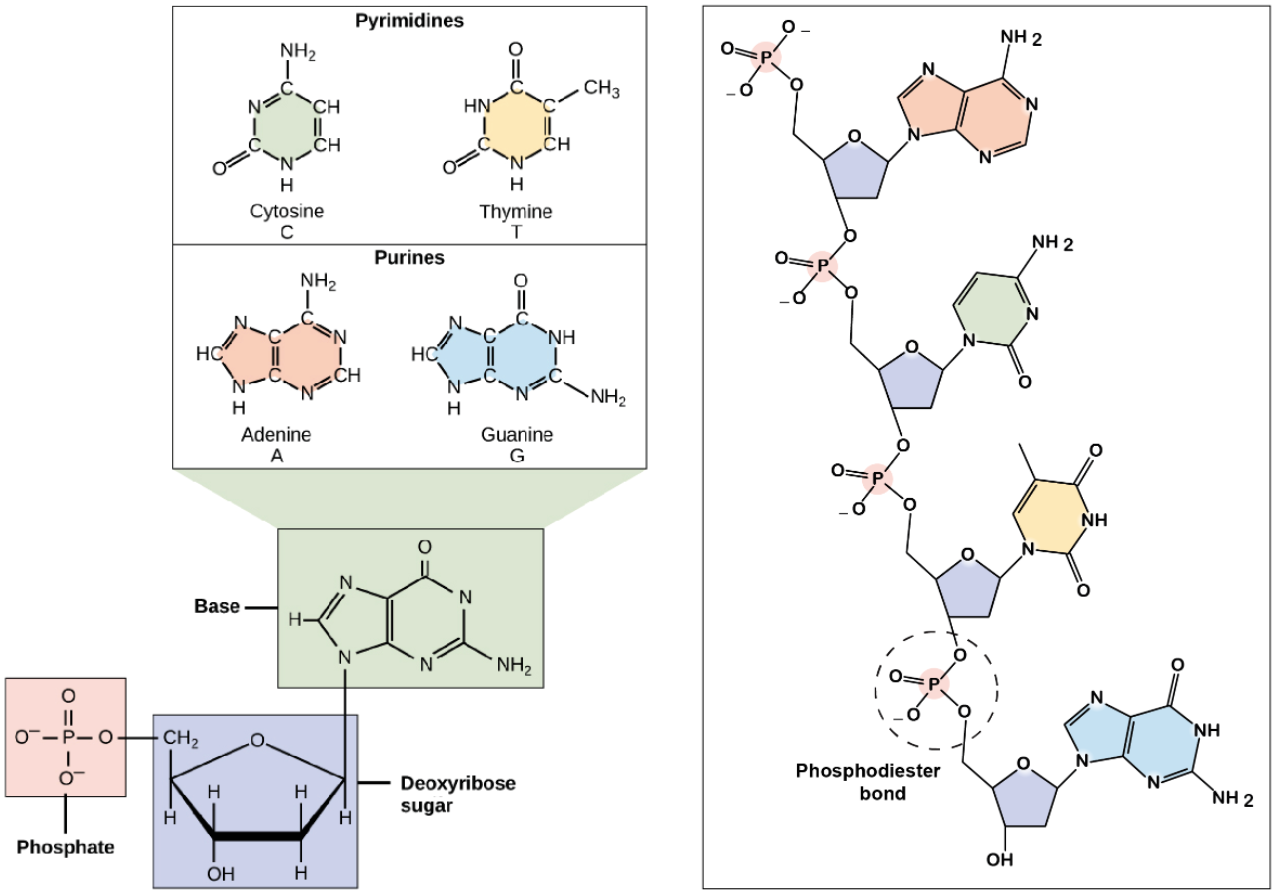
\includegraphics[width=0.9\textwidth]{dnaStruct}
\caption{\label{fig:dnaStruct}The structure of DNA. (Taken from Khan Academy)}
\end{centering}
\end{figure}

\introduce{Base pairs} Adenine and guanine bond with 2 hydrogen bonds whilst cytosine and thymine bond with 3 hydrogen bonds (and hence this bond is slightly stronger). As a result, DNA is able to form double stranded molecules with the well-known double helix structure. Note that the width of DNA is constant because each Watson-Crick base pair is between one pyrimidine and one purine. 

\introduce{Directionality} Please note that \textbf{DNA strands are directional.} There is a 3' (hydroxyl bearing) and a 5' (phophate bearing) end and whenever a double strand molecule (\emph{complex}) forms each strand is arranged in an anti-parallel manner. When a sequence of DNA is written, it is always written 5' to 3'.

\subsection{RNA}
\introduce{RNA} \emph{Ribonucleic acid} or RNA is very similar to DNA. They are composed from similar building blocks and in a similar fashion but uridine replaces thymine in DNA. Also note that the sugar used is different.

\introduce{RNA Diversity \& Stability} In the cell, RNA often exists as single strands (this is uncommon for DNA). There is significant structure diversity since each strand is able to base pair with itself. Furthermore, note that RNA is relatively unstable compared to DNA.

\subsection{Amino Acids}
\introduce{Sub-unit} Amino acids are the sub-units used to build proteins. Their structure can be seen in Fig.~\ref{fig:aminoAcidStructure}.

\begin{figure}[h!]
\begin{centering}
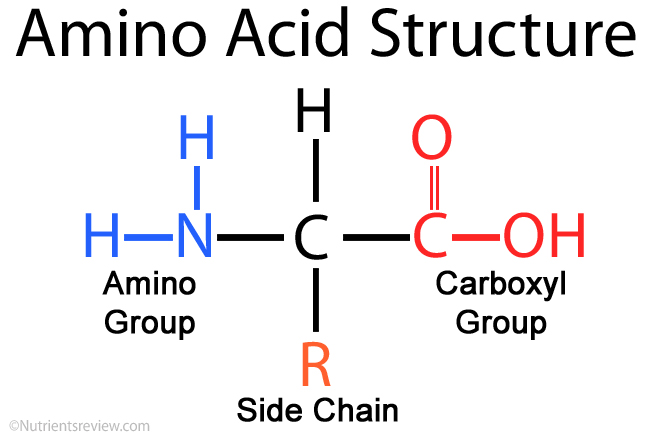
\includegraphics[width=0.3\textwidth]{aminoAcidStructure}
\caption{\label{fig:aminoAcidStructure} The structure of Amino Acids. The central carbon is referred to as the \textbf{alpha carbon} and the amino group is alkaline whilst the carboxyl group is acidic. }
\end{centering}
\end{figure}

The R group (side-chain) is different for each amino acid and effective determines the function of each amino acid. Table \ref{tab:commonAminoAcids} outlines some amino acids which are worth learning.

\begin{table}[h!]
\centering
\begin{tabular}{|p{2cm}|p{5cm}|p{3cm}|}
\hline
\textbf{Type}& \textbf{Description} & \textbf{Examples} \\ \hline
  Aliphatic   &  Do not contain especially stable carbon rings (non-aromatic).           &  Alanine, Glycine        \\ \hline
   Aromatic   &  Cyclic, planar with a ring of resonance bonds (e.g. benzene ring).      &  Tyrosine       \\ \hline
   Acidic     &  -        																 & Aspartic Acid \\  \hline
   Basic      &  -																		 & Arginine \\ \hline
   Sulfur-containing & Cysteine can form disulfide bonds; important for structure! & Cysteine\\ \hline
   Amidic & Containing a \texttt{CONH\textsubscript{2}} group. & Asparagine\\ \hline
\end{tabular}
\caption{Common Amino Acids (worth learning).}
\label{tab:commonAminoAcids}
\end{table}

\introduce{Peptide Bonds} Amino acids form proteins through polymerization; through a dehydration reaction, multiple amino acids are able to join together forming peptide bonds.
Even though the peptide bond itself is planar, the bonds around each alpha carbon are able to rotate giving great flexibility.

\subsection{Proteins}
\subsubsection*{Protein Structure}
\introduce{Secondary Structures: What \& Why?}
Hydrogen bonding between the sub-units in each polypeptide chain result in secondary structure. There are two main forms of secondary structure in proteins as seen in Fig. \ref{fig:proteinSecondaryStructure}.
\begin{enumerate}
\item Hydrogen bonding between \texttt{N-H \& C=O} four residues away cause \textbf{alpha helices} to form.
\item Hydrogen bonding between adjacent parallel or anti-parallel strands cause \textbf{beta sheets} to form.
\end{enumerate}

\begin{figure}[h!]
\begin{centering}
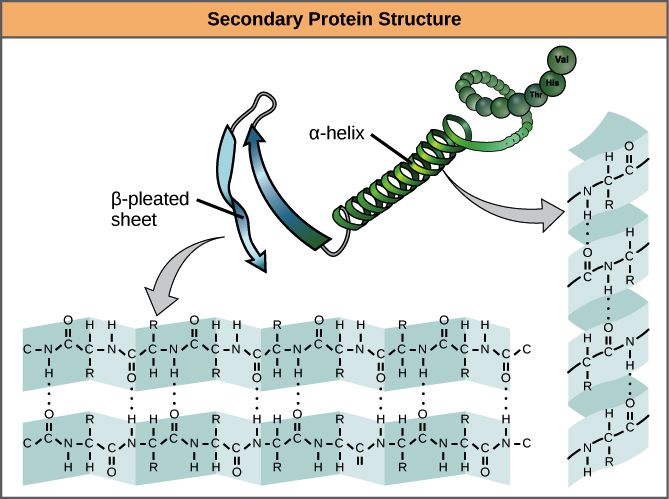
\includegraphics[width=0.6\textwidth]{proteinSecondaryStructure}
\caption{\label{fig:proteinSecondaryStructure} Protein secondary structure; hydrogen bonds shown. }
\end{centering}
\end{figure}

\introduce{Protein Structure} The structure of proteins is hierarchical. Primary structure refers to the sequence of amino acids whilst secondary structure refers to local folded structures (see above). The overall 3D structure of a polypeptide is the tertiary structure and is primarily due to interactions between different R groups. The quaternary structure only applies for proteins made up of several polypeptide chains and outlines how these chains interact (i.e. the complex formed). 

\subsubsection*{Protein Function}
\textbf{Proteins carry out a wide range of roles} in the cell such as acting as enzymes and structural roles with a high degree of specificity. For example, transmembrane transporters can distinguish between \texttt{Na\textsuperscript{+}} \& \texttt{K\textsuperscript{+}} ions.

\introduce{How?} Molecular recognition is bases on complementarity of shape and chemical properties (e.g. charge) and hence \textbf{protein shape is  critical}.

\subsection{Phospholipids}
\introduce{What are Phospholipid?} A class of lipids (soluble in non-polar solvents) which are amphiphilic i.e. possessing parts which are both hydrophilic (head) and hydrophobic (tail). Because of this property, structures which are energetically favourable can spontaneously form (self-assemble) such as those in Fig. \ref{fig:lipidSelfAssembly}.

\introduce{Bilayer Sheet}
The bilayer sheet is especially important; cells are surrounded by a lipid bilayer membrane which isolates the cell contents from the environment as it is impermeable to most ions and water soluble molcules.

\begin{figure}[h!]
\begin{centering}
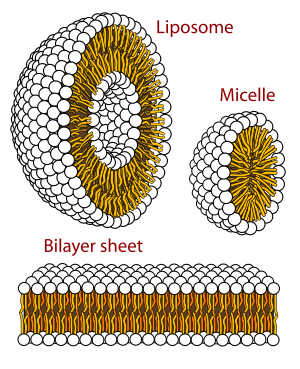
\includegraphics[width=0.3\textwidth]{lipidSelfAssembly}
\caption{\label{fig:lipidSelfAssembly} Structures formed from self-assembly}
\end{centering}
\end{figure}

\subsection*{Self-Organisation}
\introduce{Self-Organisation!} In fact, living systems in general are highly sophisticated and self-organising. In addition to phospholipids, RNA and proteins also self-assemble into complex, defined functional forms as does DNA. In fact, this self-assembly of DNA can be used to build complex structures.

\subsection{The Three Domain System}
\introduce{Three Domains} When organising species, the domain is the highest rank of species used. Bacteria \& archea  are prokaryotes i.e. single celled and lacking a membrane bound nucleus whilst eukaryotes have nuclei and other organelles with membranes.

\subsubsection*{Archea}
Archea were originally classed as bacteria. They are though of as extremophiles which inhabit as diverse environments as bacteria. They have similar metabolic pathways to eubacteria (bacteria with rigid cell walls) but some enzymes are more similar to those of eukaryotes.

\introduce{Relevance} They play important roles in the carbon and nitrogen cycle and do not act as parasites. Their robustness and metabolism is useful for \textbf{biotechnology}.

\subsubsection*{Bacteria}
Bacteria are found almost everywhere and are a significant proportion of the worlds biomass. They have no nucleus.

\introduce{Relevance} They are critical to nutrient cycles. Bacteria are important for good health but also responsible for many diseases.

\subsubsection*{Eukaryotes}
Eukaryotes have both single and multicellular forms with a large array of different physical forms. They inhabit diverse diverse environments and include plants, animals and fungi. Animals and plants are both eukarya and Fig. \ref{fig:animalVsPlant} shows some of the differences between their cells.

\introduce{Relevance} We are eukarya! They are capable of significant environmental impact and many are of great importance to our survival.

\subsubsection*{Genetic Organisation}
\introduce{Prokaryotes} Prokaryotes typically have a single circular chromosome with extrachromosomal elements known as plasmids which form the basis for cloning vectors.

\introduce{Eukaryotes} Eukaryotes typically have several linear chromosomes. Within their cells, mitochondria and chloroplasts have their own DNA and some `lower forms' can have plasmids.

\introduce{Chromosome Packing} DNA is wrapped around \textbf{histones} (proteins which bind with DNA through electrostatic interactions) to form a nucleosome which is the building block of chromatin. Nucleosomes coil to form chromatin fibres which are condensed into chromosomes during cell division. Note that the packing is dynamic according to the needs to the cell. See Fig. \ref{fig:chromoPacking} to understand the hierarchical packing of chromosomes. 

\introduce{Centromeres and Telomere}Also note that chromosomes have centromeres (where chromosomes attach to the spindle during cell division - the central part of the chromosome) and telomeres at the end. 

\begin{figure}[h!]
\begin{centering}
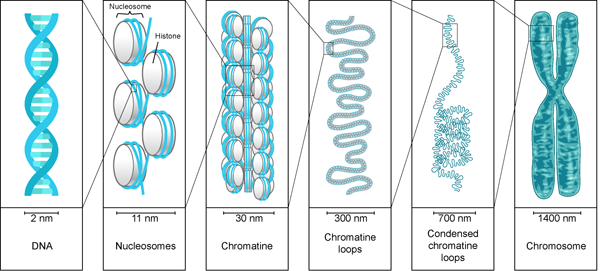
\includegraphics[width=0.7\textwidth]{chromosomePacking}
\caption{\label{fig:chromoPacking} Chromosome Packing }
\end{centering}
\end{figure}

\subsection{Antibodies}
Antibobies are proteins which are used naturally to neutralise pathogens. They have several useful properties. \ix{Properties}
\begin{itemize}
\item They are able to recognise antigens (protein coatings) which a very high degree of specificity.
\item They are highly diverse, aided by the combination of light and heavy chains. 
\item They are robust and long-lived; disulfide bonds help to prevent degradation.
\item They are bivalent. 
\end{itemize}

\ix{Antibody Structure}
\begin{figure}[H]
\begin{centering}
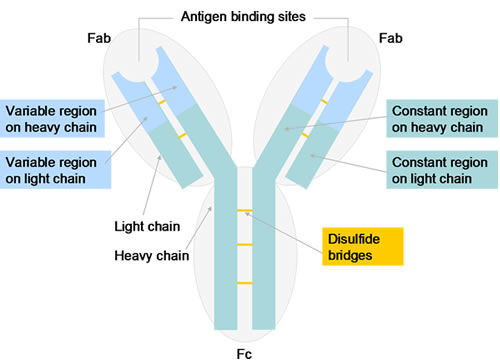
\includegraphics[width=0.5\textwidth]{antibodyStructure}
\caption{\label{fig:antibodyStructure} Structure of Antibodies. Fab: Fragment antigen binding. Fc: Fragment crystallisable.}
\end{centering}
\end{figure}

There are antibody isotype\ix{Isotypes} determined by the constant regions which determine how antibodies interact with each other. Each class is linked to a specific gene. For example, \texttt{IgA} is produced using gene $\alpha$ and \texttt{IgG} is produced using gene $\gamma$ (the remaining types follow this pattern). Each isotype is found in different places in the body and they act in different ways. 

\begin{figure}[H]
\begin{centering}
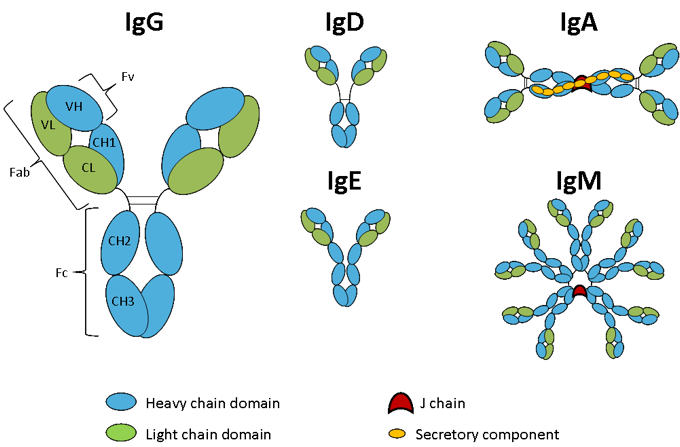
\includegraphics[width=0.5\textwidth]{antibodyIsotypes}
\caption{\label{fig:antibodyIsotypes} Different antibody isotypes. They contain different constant regions, leading to different complexes.}
\end{centering}
\end{figure}

The \ix{CDR} complementarity-determining regions are part of the variable chains where the molecules specifically bind to their antigen and as the name suggests, variable chains change between antibodies.

There is significant antibody diversity due to \ix{Somatic/VDJ}\textbf{somatic recombination}. The variable region of each chain encoded in several gene segments of which there are three types, V (variable), D (diversity) \& J (joining) (note, no D segments in light chains). Each B cell (a type of white blood cells of the lymphocyte subtype which secrets one type of antibody) will assemble a variable region by \textbf{randomly selecting and combining one V, D \& J segment.} This leads to a very large number of different antibodies.

\begin{figure}[H]
\begin{centering}
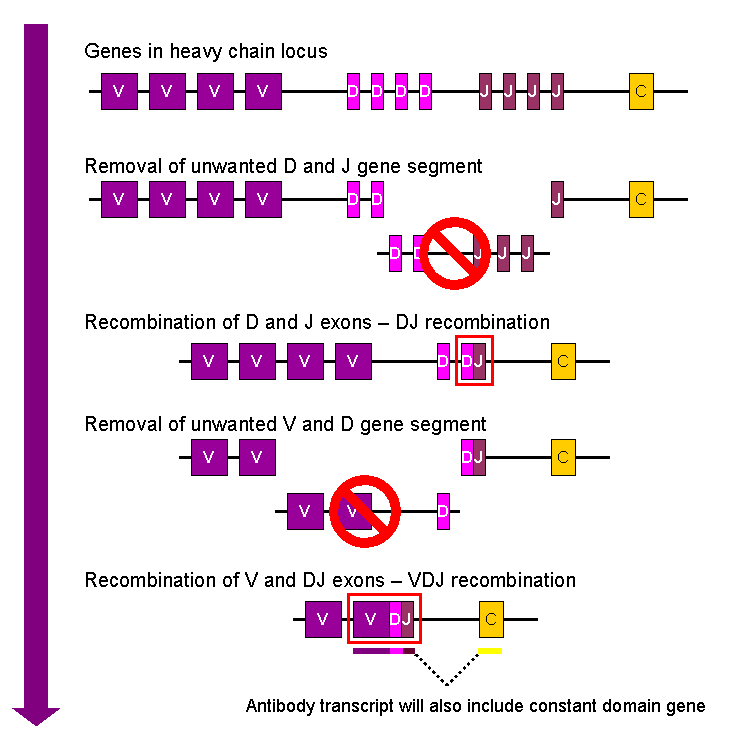
\includegraphics[width=0.6\textwidth]{vdjRecomb}
\caption{\label{fig:vdfRecomb} Somatic/VDJ recombination.}
\end{centering}
\end{figure}

B cells are able to switch their class\ix{Class Switching}, changing the isotype of antibody they produce e.g. from \texttt{IgM} to \texttt{IgG}. The \textbf{constant-region of the heavy chain is changed but the variable region remains constant} meaning that \textbf{class switching does not affect antibody specificity}. Please note that only one heavy chain and one light chain is expressed within each B cell.

\begin{figure}[H]
\begin{centering}
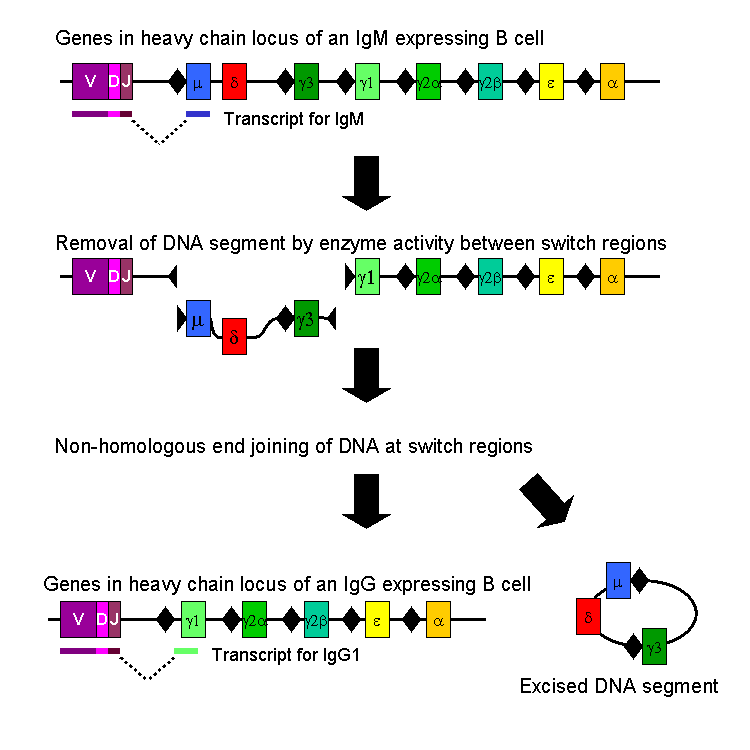
\includegraphics[width=0.6\textwidth]{antibodyClassSwitching}
\caption{\label{fig:absClassSwitching} Recombination for B cell class switching.}
\end{centering}
\end{figure}

\subsection{Eukaryotic Cell Division}
Cell division is essential for life. There are two primary forms of eukaryotic cell division.
\subsubsection*{Mitosis}
\introduce{Mitosis} Mitosis creates clones of an original diploid cell by copying each chromosome and then splitting the cell. NB: The chromosomes are seperated using a microtubule spindle.

\begin{figure}[h!]
\begin{centering}
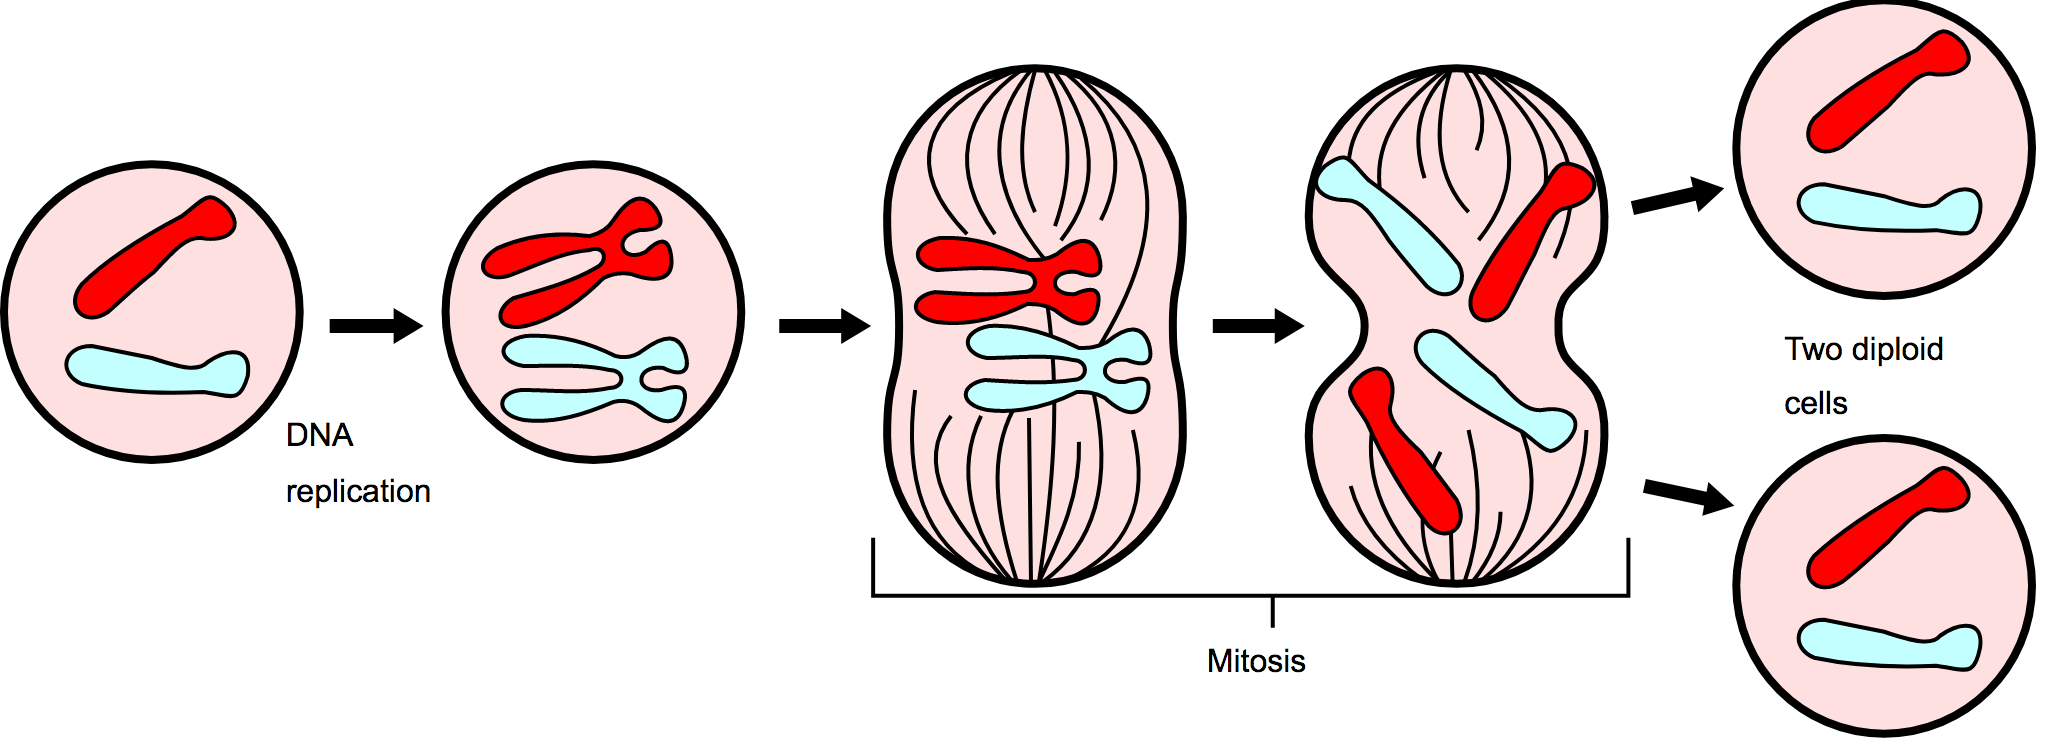
\includegraphics[width=0.7\textwidth]{mitosis}
\caption{\label{fig:mitosis} Mitosis.}
\end{centering}
\end{figure}

\subsubsection*{Meiosis}
\introduce{Meiosis} Meiosis is a \emph{reductive} type of cell division which forms \textbf{haploid gametes} - cells with single copies of DNA which are able to unite with another cell of the opposite sex during reproduction. Hence meiosis is part of the sexual life cycle. Fig. \ref{fig:meiosis} outlines how meiosis occurs; note that crossing over occurs.

\introduce{Recombination} Gamete recombination is important as it creates new combinations of alleles (different forms of the same gene).

\begin{figure}[h!]
\begin{centering}
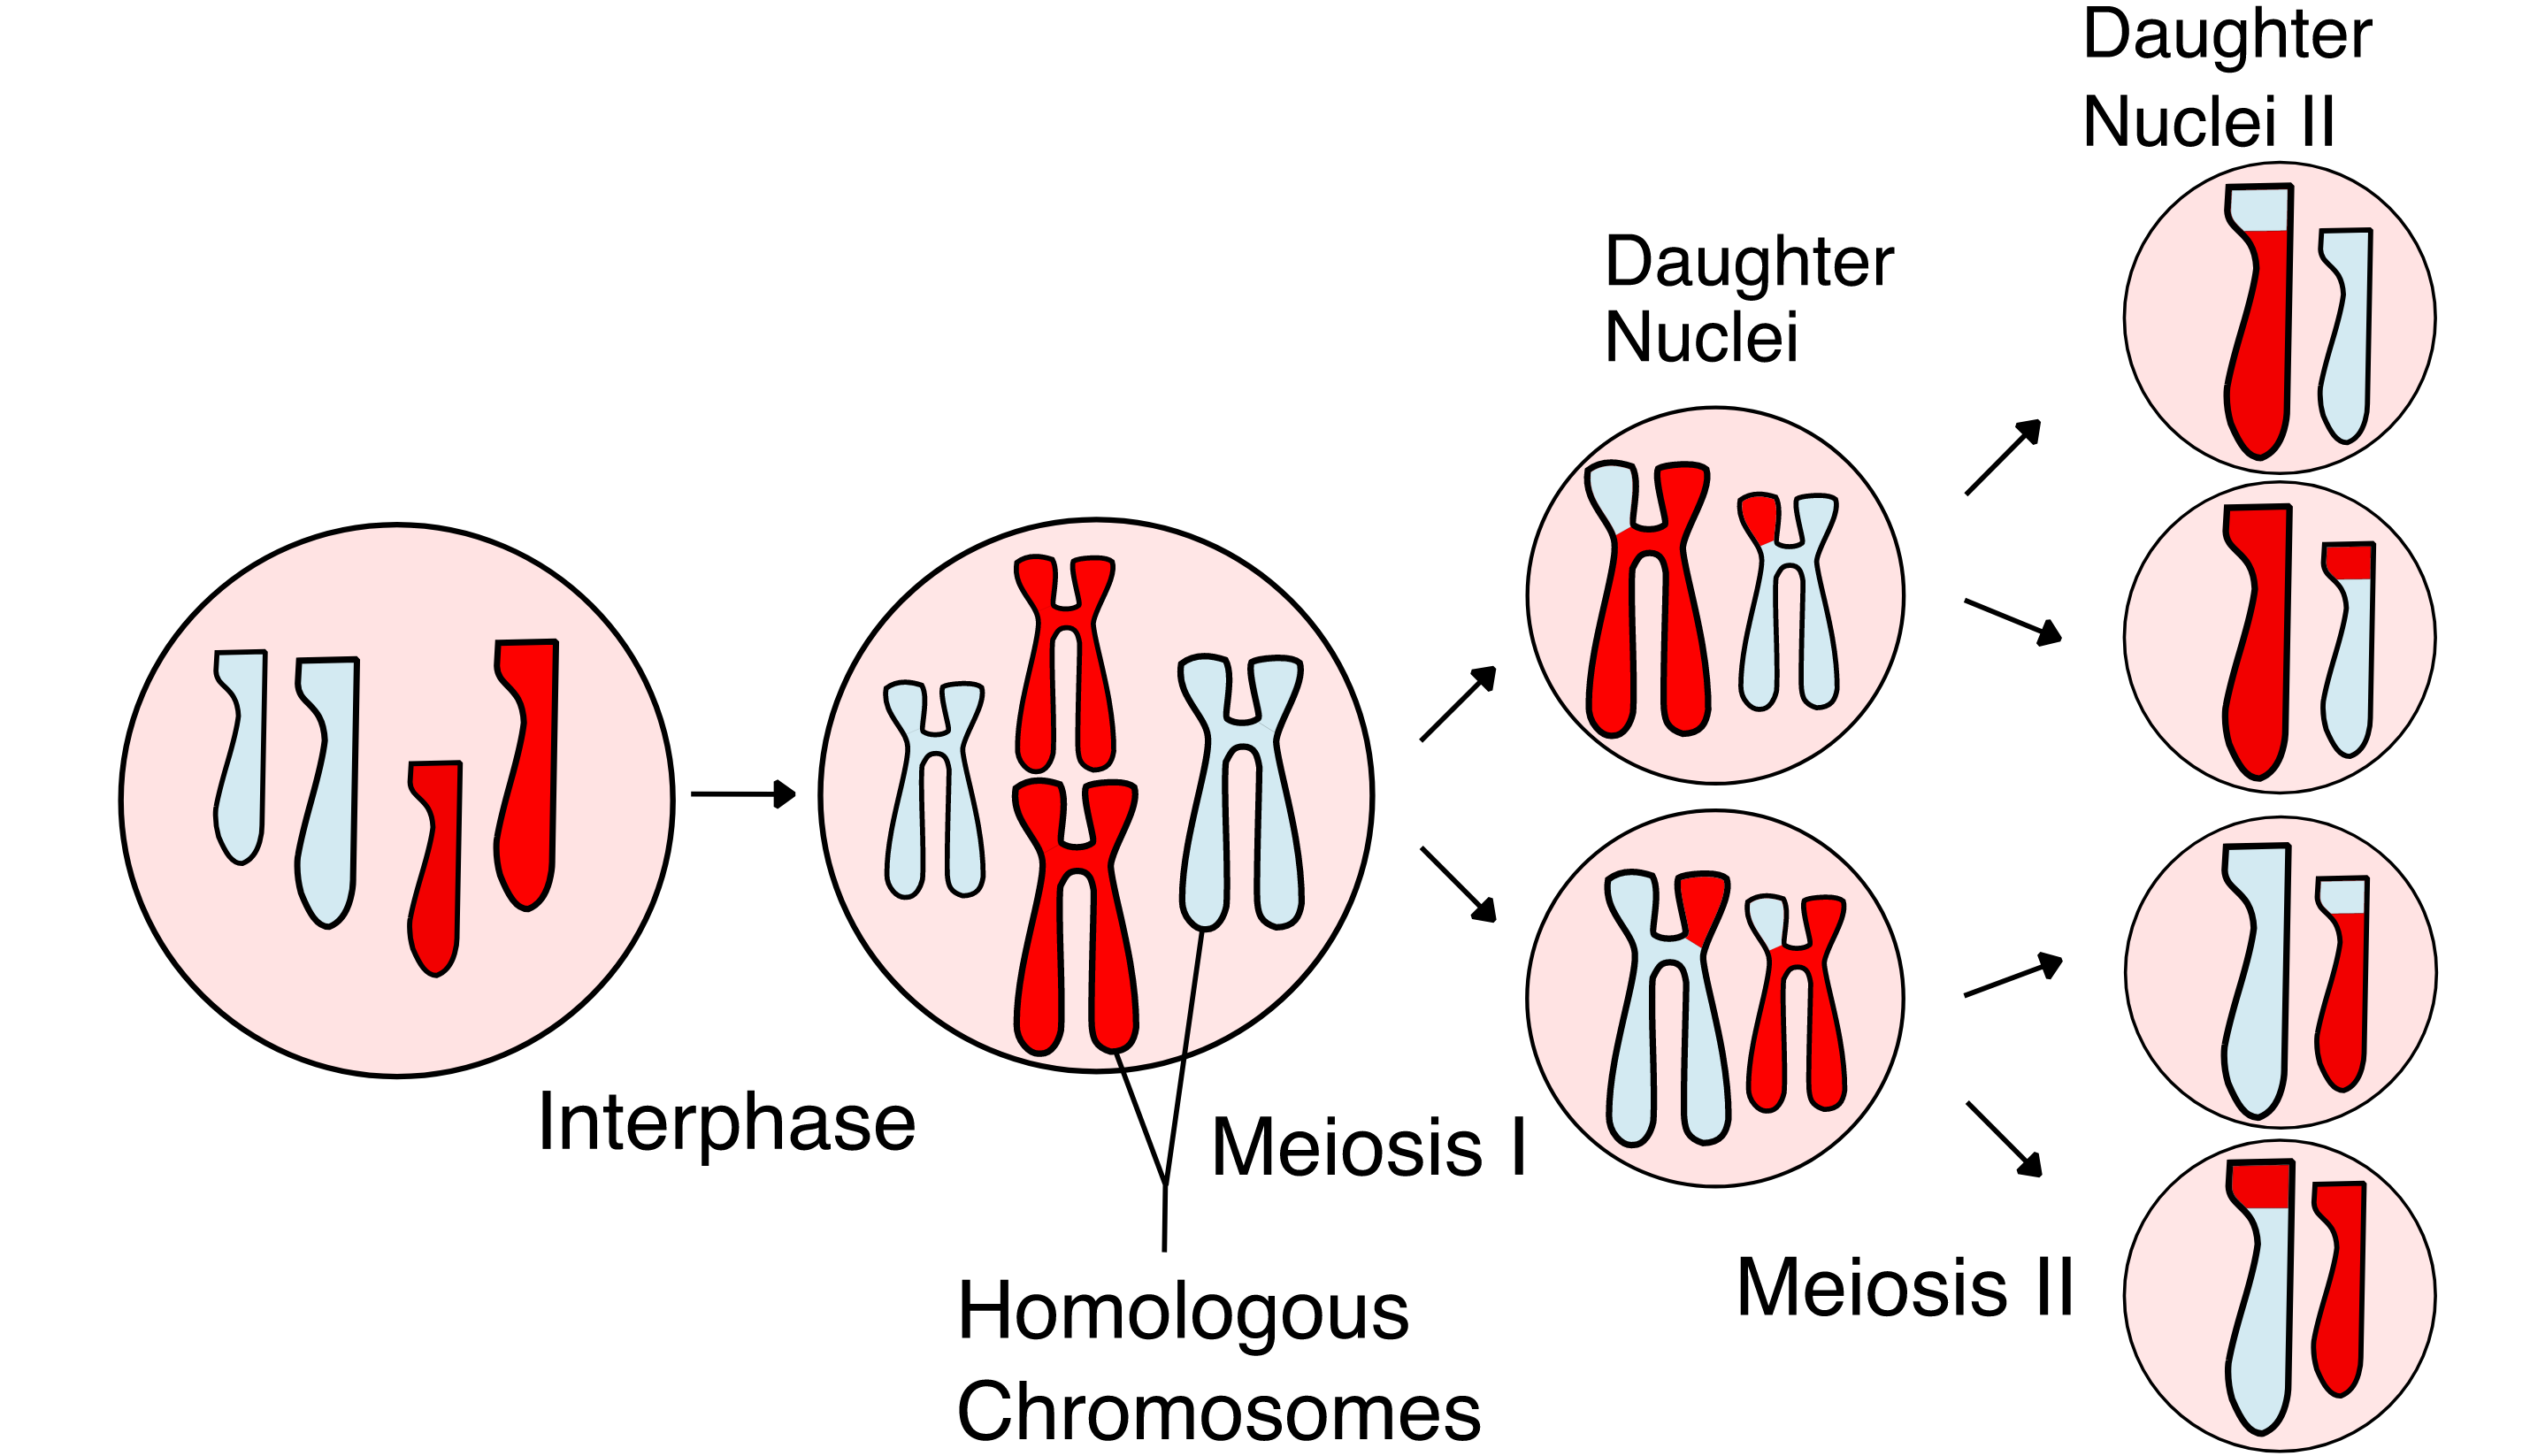
\includegraphics[width=0.7\textwidth]{meiosis}
\caption{\label{fig:meiosis} Meiosis.}
\end{centering}
\end{figure}

\section{The Central Dogma}
\subsection{The Central Dogma of Molecular Biology}
\introduce{The Central Dogma}The central dogma of molecular biology is a proposed \textbf{information flow} which explains how the cell transforms encoded information into the proteins required for development and metabolic demands.
\begin{quote}
\centering
DNA $\rightarrow$ RNA $\rightarrow$ Protein
\end{quote}

\introduce{Experimental Methods Used} It had been known that there existed heritable traits for some time (e.g. Mendel 1860 \& Griffith 1928) but the molecule of heredity was unknown. It was discovered that \textbf{DNA is the molecule of heredity} by fractionating cell-free extract of S-strain cells and testing for transformation of R-strain cells (Avery, MacLeod \& McCarthy, 1944) and this was confirmed in 1952 using radioactively labeled phage; bacteria was infected with phage with radioactive \texttt{S} on the phage protein coating and radioactive \texttt{P} in phage DNA. Radioactivity was recovered primarily on phage ghosts in the first case and in the bacteria in the second case (Hershey \& Chase, 1952).

\subsection{DNA Replication}
If DNA is the molecule of heredity, DNA must be able to replicate.

\introduce{Adding Deoxynucleotides} \textbf{Using a template strand,} an additional nucleotide can be added in two stages. First, a nucleotide forms hydrogen bonds with the exposed base on the template strand and then \textbf{DNA Polymerase} creates a phosphodiester bond between the adjacent nucleotides on the non-template strand. This process only occurs in a buffer solution at the correct pH. \introduce{A caveat...} However, note that \textbf{DNA Polymerase only works from 5' to 3'}! Hence synthesis of the lagging strand is discontinuous and there are \textbf{okazaki} fragments.

\introduce{How does DNA replicate?} A double helix replicates by separating the helix into each strand and then cloning each strand, which can be shown by growing bacteria in a heavy \texttt{N} media and switching to grow in a normal \texttt{N} and observing that there exist DNA molecules with both heavy and light \texttt{N} (Meselson \& Stahl, 1958). \textbf{N.B. DNA can be seperated using density gradient centrifugation.}

\begin{figure}[h!]
\begin{centering}
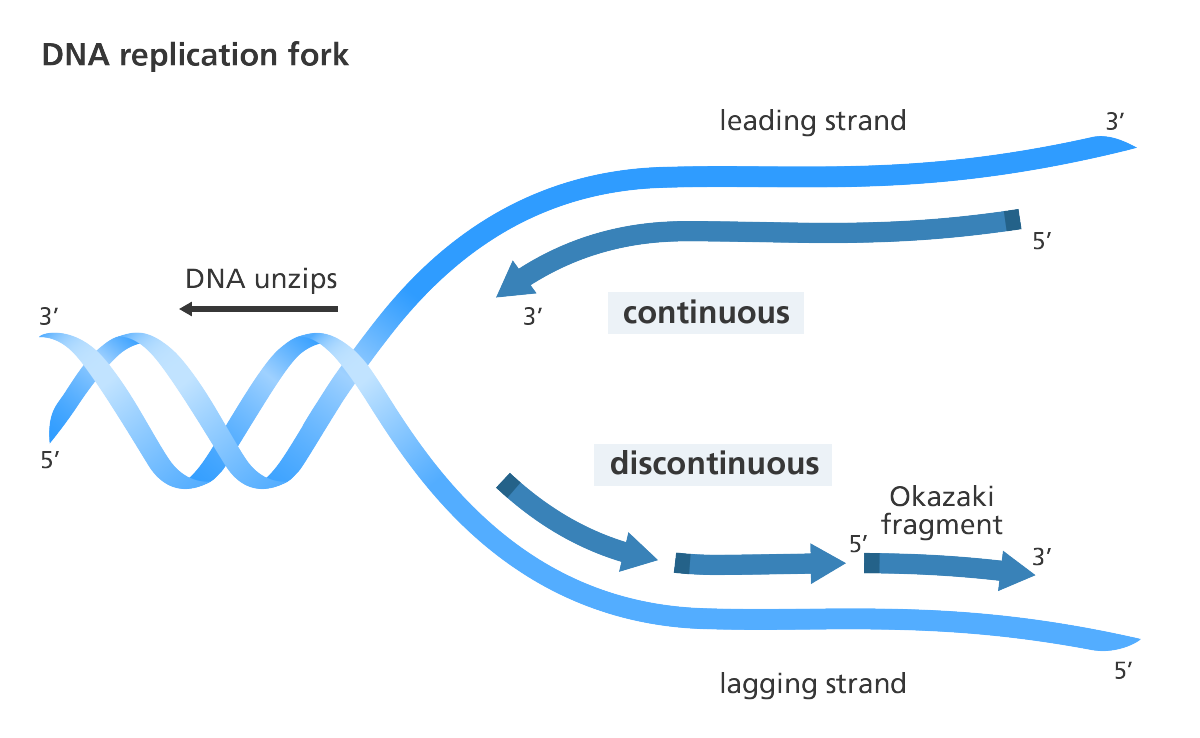
\includegraphics[width=0.8\textwidth]{dnaReplication}
\caption{\label{fig:dnaReplication} DNA Replication}
\end{centering}
\end{figure}

Several enzymes are essential for DNA replication including but not limited to the following:  \introduce{Enzymes involved}
\begin{itemize}
\item DNA Polymerase III is essential for DNA replication and adds phosphodiester bonds between nucleotides.
\item DNA Helicase is responsible for seperating the double-stranded DNA.
\item RNA Primase places RNA primer as DNA Polymerase III requires a double stranded region to begin replicating DNA.
\item Topoisomerase is responsible for unwinding the DNA.
\item DNA Ligase repairs breaks in DNA strands (e.g. due to okazaki fragments).
\end{itemize}

\subsection{RNA as a Messenger}
Short-lived RNA was observed and was hypothesised to encode for information. \textbf{DNA is transcribed to} \textbf{messenger RNA} mRNA which conveys genetic information to the ribosome. \introduce{Transcription} RNA polymerase synthesises RNA using a template strand but note that only one strand is used; hence there is a template strand and a coding strand (but note that \texttt{U} replaces \texttt{T}).

\begin{figure}[h!]
\begin{centering}
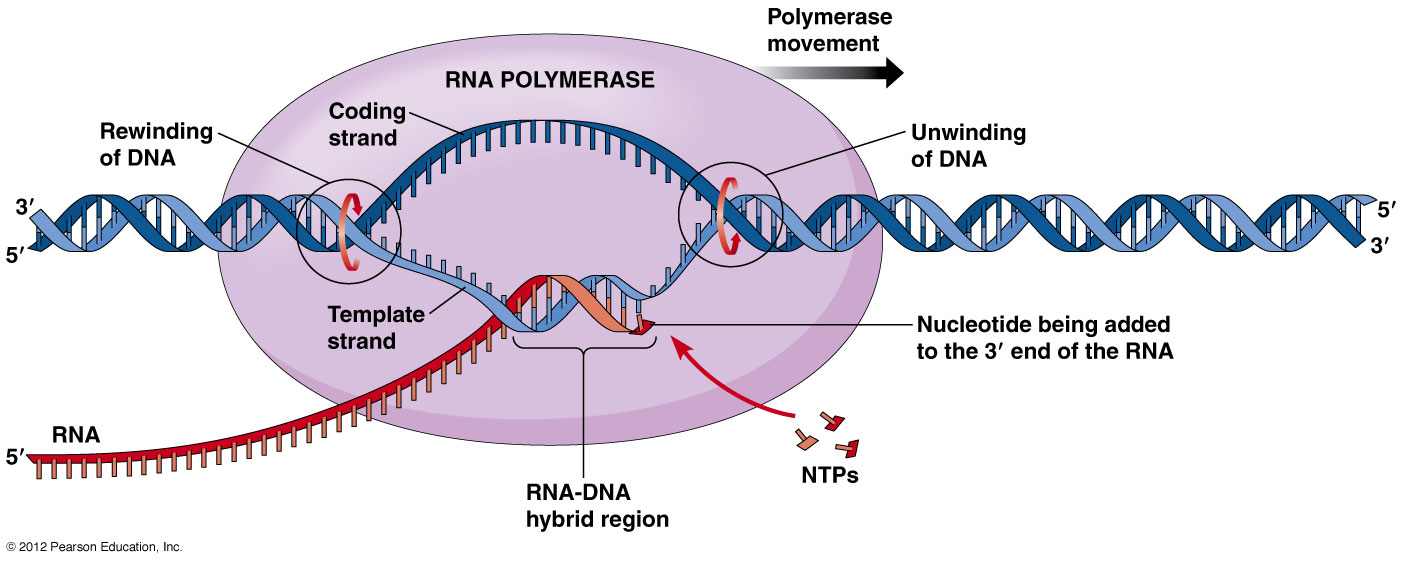
\includegraphics[width=\textwidth]{rnaTranscription}
\caption{\label{fig:rnaTranscription} RNA Transcription}
\end{centering}
\end{figure}

\subsection{Translation}
The \introduce{Code Used}triplet code was suggested since this gave $4^3=64$ different amino acids and there needed to be at least 20 (i.e. the 20 common amino acids). Each \textbf{triplet is called a codon} and there are multiple codons coding for the same amino acid. Note that \texttt{AUG} is the most common start codon (which also codes for methionine) and \texttt{UAG}, \texttt{UAA}, \texttt{UGA} are stop codons (which do not specify amino acids).

Ribosomes\introduce{Ribosomes} are the structures where polypeptides are build anad are made up of protein and ribosomal RNA (rRNA). The ribosome not only acts as an enzyme for protein synthesis but also structurally aids each tRNA to find its matching codon.

\textbf{Transfer RNAs}\introduce{Transfer RNAs} are molecular bridges that connect mRNA codons to the amino acids they encode. Each tRNA has an anticodon which is able to bind to the mRNA and the other end of the tRNA carries the amino acid specified by the codon. One way of observed this is to radioactively label different tRNAs (which would then bind to different codons) and add to washed ribosomes complexed with known mRNA, then filtering out the ribosome and noting where radioactivity is found(Nirenberg \& Leder, 1964).
\begin{figure}[h!]
\begin{centering}
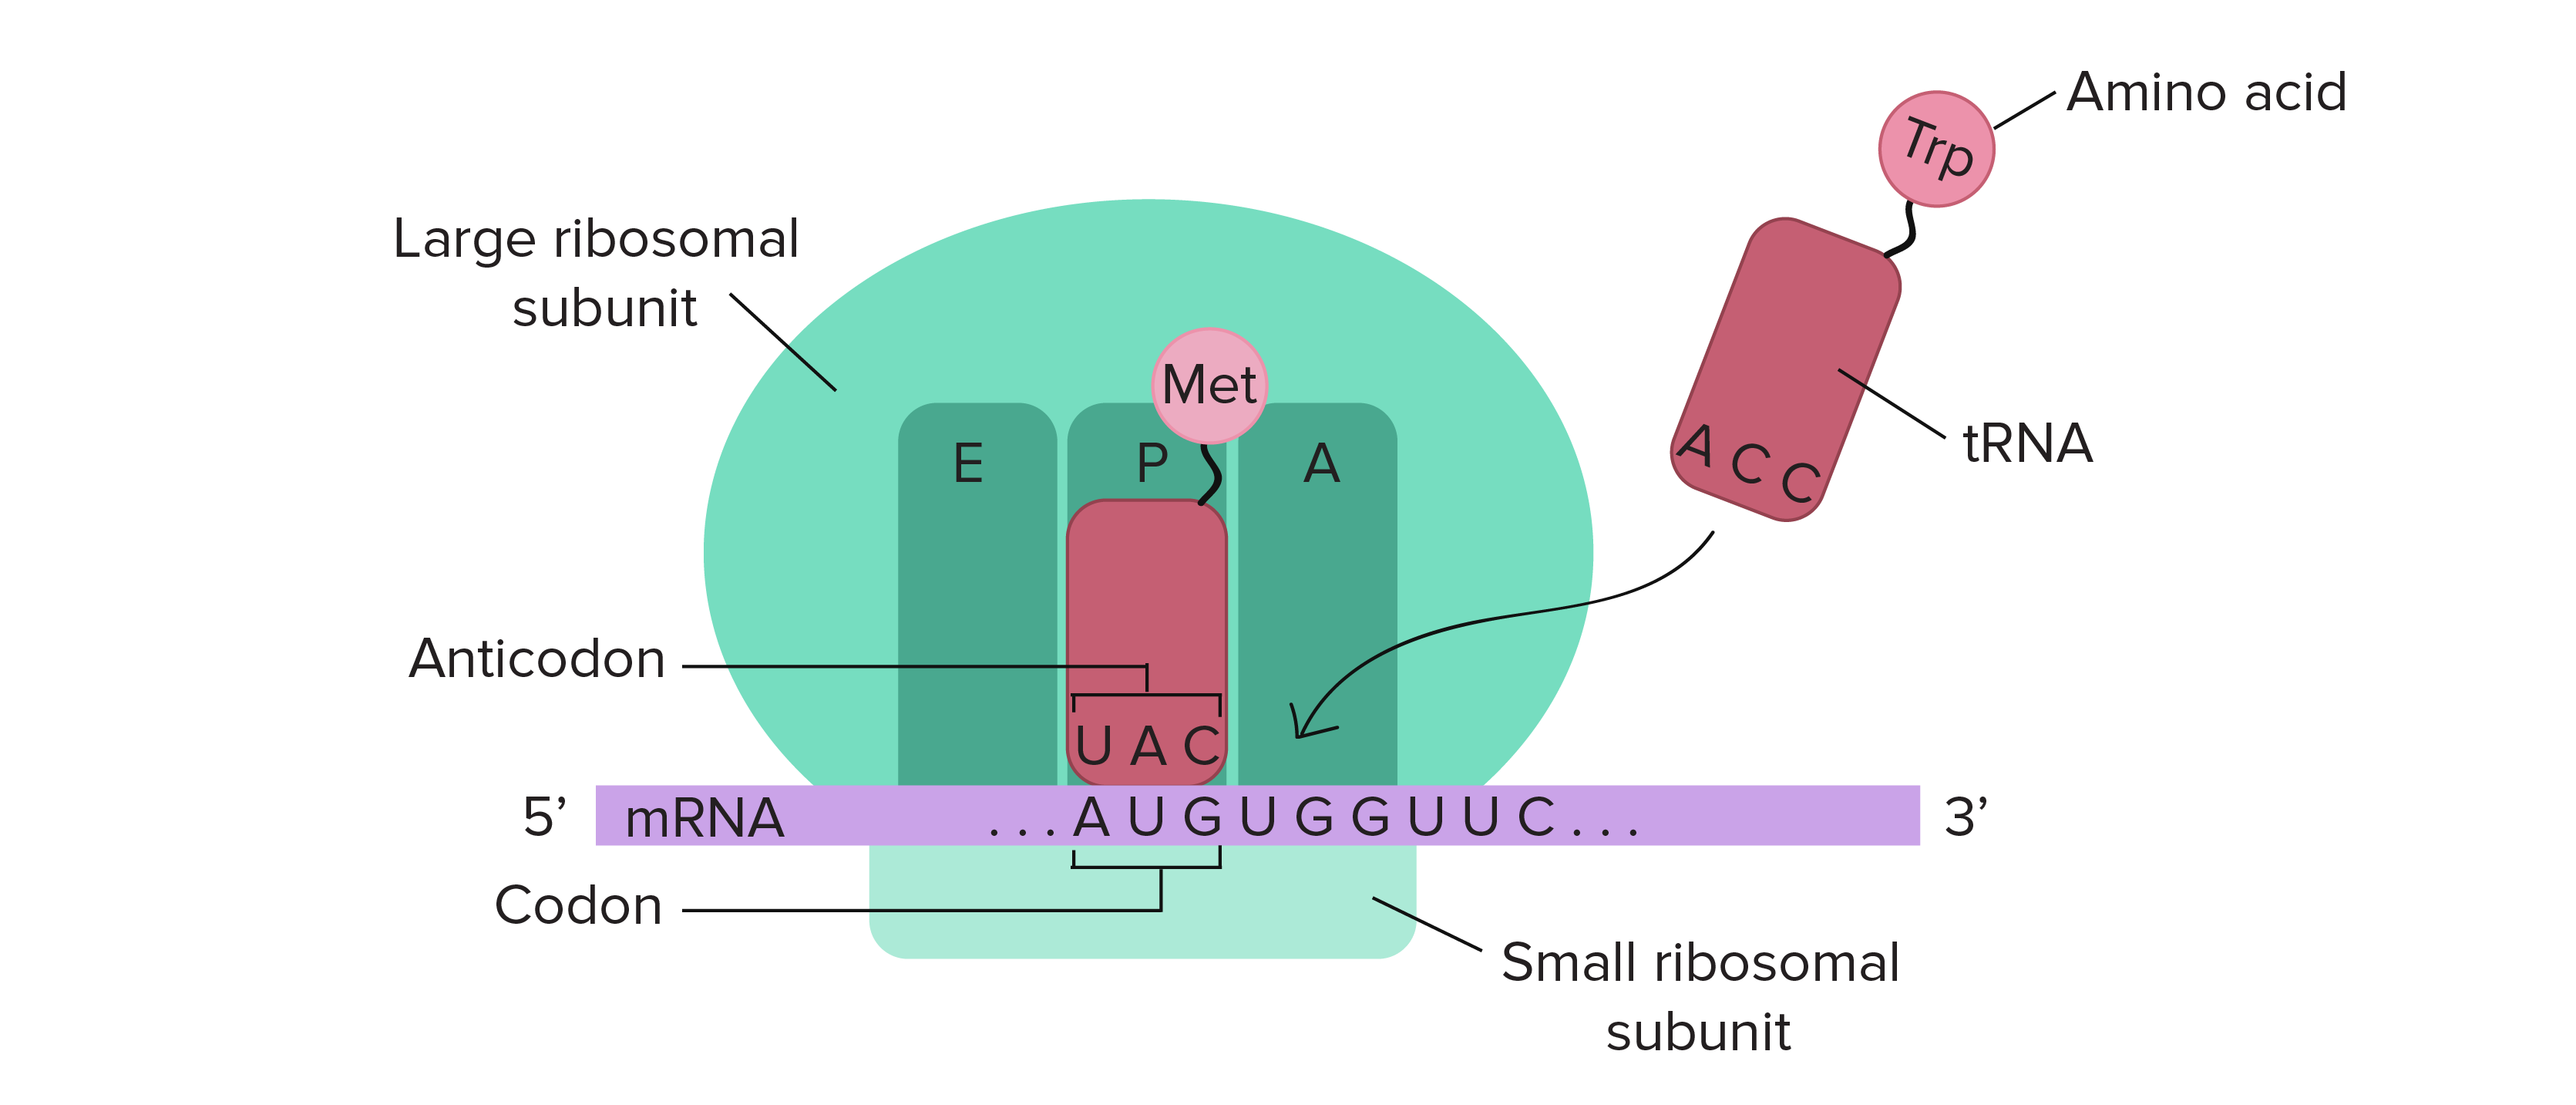
\includegraphics[width=\textwidth]{translationTRNA}
\caption{\label{fig:translationTRNA} tRNA use.}
\end{centering}
\end{figure}

Each tRNA\introduce{Wobble Base Pair} can read one \textbf{or multiple codons}; Crick suggested that the third base was less spatiailly contrained than the previous two base pairs and hence can have non-standard (wobble) base pairs. Hence whilst there are 61 possible tRNAs, many cells have fewer due to the wobble base pairs with a minimum of 31 for unambiguous translation.

In prokaryoes\ix{Prokaryotic Translation}, translation occurs simultaneously with transcription. However, in eukaryotics the translation product may pass into the endoplasmic retriculum for cleavage of signal peptides. Once passed to the Golgi complex, further processing occurs and eventually the peptide can be secreted.


\section{Gene Control}
\subsection{General Structure}
The structure of DNA sequences in the genome is important.
\begin{figure}[h!]
\begin{centering}
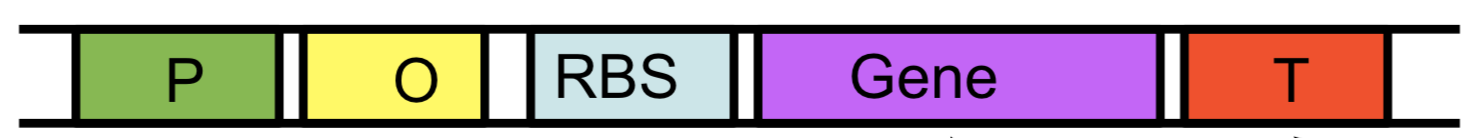
\includegraphics[width=0.8\textwidth]{generalStructure}
\caption{\label{fig:generalStructure} The structure of \textbf{genes? Is this the right word?}}
\end{centering}
\end{figure}
There are several components:
\begin{itemize}
\item The promotor is the region of DNA that initiates transcription of a gene and where RNA polymerase is able to find. They can also be regulated.
\item The operator is a region of DNA made up of binding sites for repressor protein and other transcription factors / regulatory elements.
\item The ribsome binding site is the location in mRNA where the the ribosome binds and translation starts.
\item The gene is the protein coding sequence.
\item The terminator is the mRNA location where transcription terminates e.g. a hairpin in mRNA.
\end{itemize}

\subsection{The \emph{E. Coli lac} operon}
For many bacteria, glucose is the prefered carbon source and the ability to use other sugars is carefully controlled. The cell is able to use lactose and the \emph{lac} operon controls the use of lactose depending on the amounts of both lactose and glucose present.

\begin{figure}[h!]
\begin{centering}
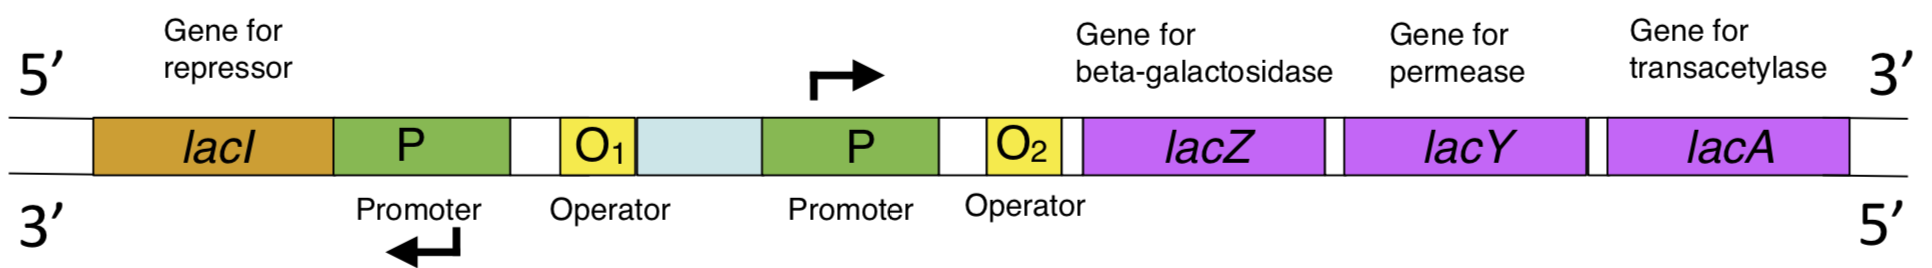
\includegraphics[width=\textwidth]{lacOperon}
\caption{\label{fig:lacOperon} The structure of the \emph{lac} operon, noting that ribosome binding sites and other encoding sequences are left out.}
\end{centering}
\end{figure}

It is important to understand what each gene codes for:
\begin{itemize}
\item\emph{lacI}\introduce{lacI} codes for the repressor protein.
\item\emph{lacZ}\introduce{lacZ} codes for beta-galactosidase which hydrolyses lactose into allolactose as well as glucose \& galactose.
\item\emph{lacY}\introduce{lacY} codes for permease which allows more lactose to enter the cell.
\item\emph{lacA}\introduce{lacA} codes for transacetylase whose biological role remains unclear.
\end{itemize}

Note a few key elements of the lac operon:
\begin{itemize}
\item The \textbf{promotor} is where RNA polymerase binds and hence where transcription begins. They may be \emph{constitutive} or regulated. 
\item The \textbf{operator} regions are bound together by the \emph{lac} repressor protein if present. When this occurs, RNA polymerase is unable to bind to the promoter.
\item Cyclic AMP (adenosine monophosphate) binds to CRP (cAMP receptor protein, also known as catabolite activator protein) allowing the CAP binds to the CAP binding site (blue, note that this is only possible when cAMP is bound to CAP). When CAP is bound to this site, transcription is promoted by aiding the binding of RNA polymerase.
\end{itemize}

The conditions which the \emph{lac} operon operators under are very important.
\begin{itemize}
\item Without lactose, since the operator regions are bound by the repressor there is only a \textbf{low level `leaky' expression}\introduce{Leak} of \emph{lacZ} e.t.c since this complex is in fact in equilibrium with an unbound complex.

\item In the presence of Lactose\introduce{Lactose}, allolactose created by hydrolysis of lactose is able to induce the \emph{lac} operon by binding to the repressor protein. There is positive feedback as this results in the synthesis of permease which allows further allolactose into the cell.

\item The amount of cyclic AMP is inversely proportional to the glucose in the bacterial cell.\introduce{Glucose} Hence as glucose levels rise, the amount of cyclic AMP in the cells fall and hence the activity of the lac operon falls; this is negative feedback. With high levels of glucose, transcription only occurs at a low level.
\end{itemize}

Hence, the lactose operon serves to regulate the use of lactose in the cell depending on the amount of glucose (and lactose) present.

\subsection{The \emph{ars} operon}
The ars operon is an example of negative auto regulation i.e. self-regulation. The Arsenic repressor respresses its own transcription in the absence of arsenic.

\begin{figure}[h!]
\begin{center}
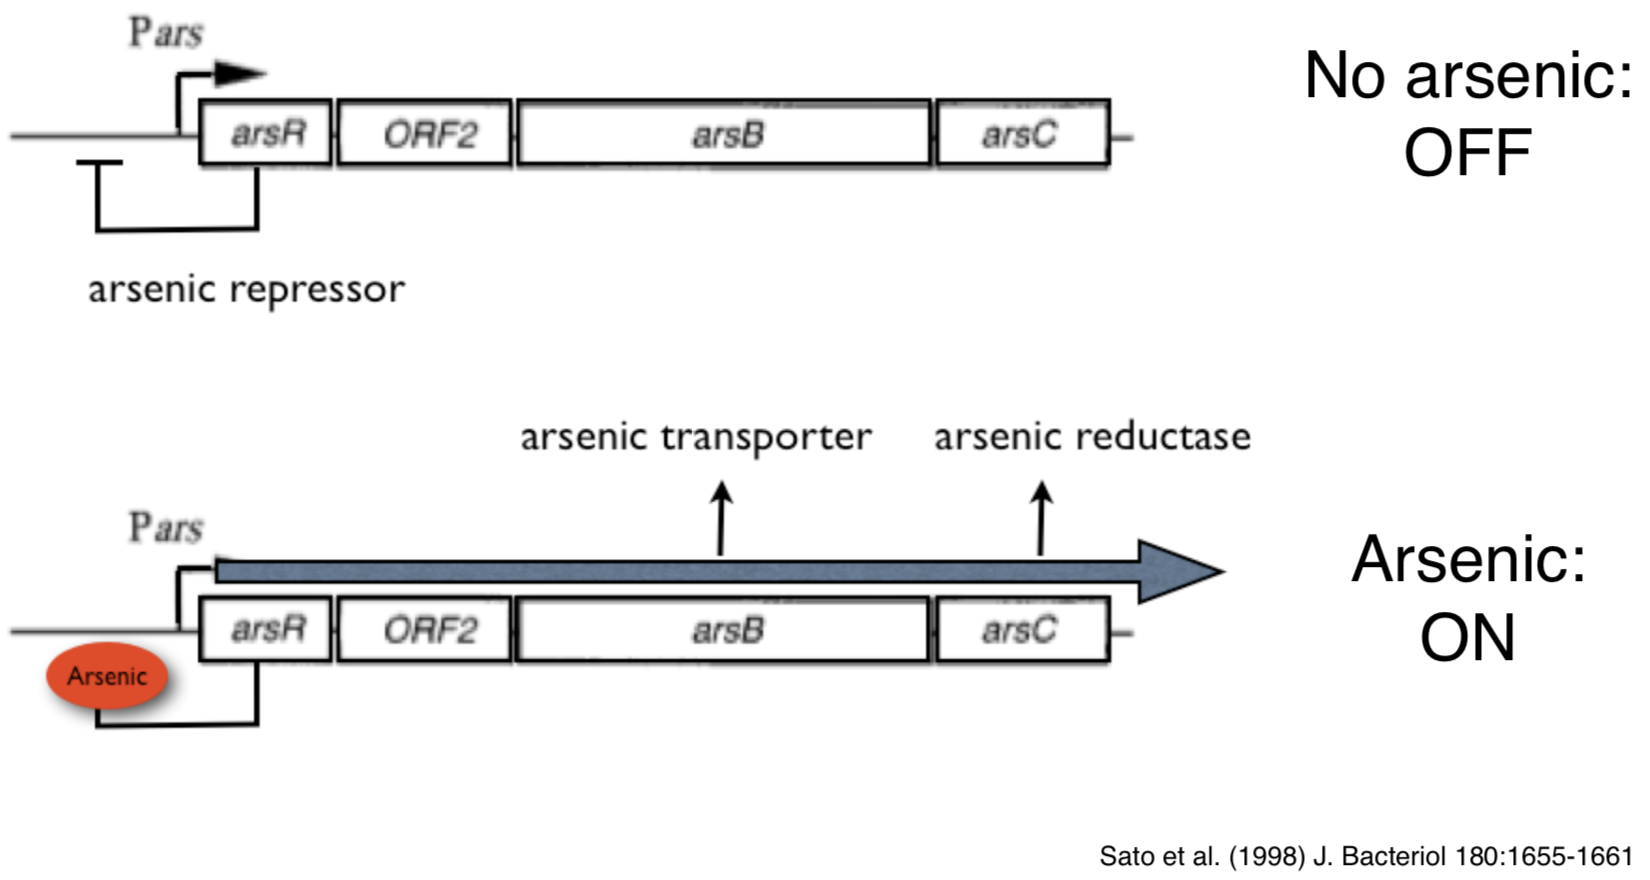
\includegraphics[width=0.7\textwidth]{arsOperon}
\end{center}
\end{figure}

\section{Genetic Engineering}
\subsection{Molecular Cloning}
\subsubsection*{Cutting \& Pasting DNA}
Restriction Enzymes\introduce{Cutting DNA}, a bacterial defense mechanism, are able to cut out DNA. They cut at specific recognition sites whose sequences are often palindromic. Some Restriction\introduce{Ends} enzymes create DNA with \emph{sticky ends} (longer sections of overhanging DNA) whilst other enzymes produce blunt ends (no overhanging DNA). Note that chromosomal\introduce{Chromosomal DNA} DNA is protected by a DNA \emph{methylase}


\textbf{DNA Ligase}\introduce{Pasting DNA} repairs breaks in double stranded DNA and is hence used to `paste' DNA segments together producing recombinant DNA.

\subsubsection*{Separating DNA}
Gel\introduce{Technique for Separation} electrophoresis can be used to separate DNA molecules.

Since\introduce{Methodology} DNA is negatively charged in solutions at pH $7-8$, it will move in an electric field. Smaller molecules will migrate more rapidly. DNA can be visualised under UV light by staining with dyes e.g. ethidium bromide.

\subsubsection*{Transforming DNA}
Modified DNA needs to be taken up by the cell. There are two methods for doing this and in each case the cells are allowed to recover before selection occurs.
\begin{enumerate}
\item\underline{Chemical Transformation}\introduce{Chemical Transformation}. Cells are chilled in \texttt{CaCl\textsubscript{2}} to permeabilise the membrane. A heat shock ($\sim 42 \degree C, 30s$) prompts the uptake of new DNA.

\item\underline{Electroporation}\introduce{Electroporation}. Cells are purified to remove ions and a high voltage shock is used to punch holes in the membrane.
\end{enumerate}
Growing cell cultures on agar plates allows for isolation of each colony.

\subsubsection*{Overall Method}
We seek to isolate, propagate and and clone large quantity of particular DNA sequences. We use cloning vectors\introduce{Cloning Vector} which include endogenous plasmids, bacteriophages and bacterial artificial chromosomes to store DNA which will be taken up by the cell. The cloning vectors may include a multiple cloning site (MCS) which contains many restriction sites. Selectable markers are often introduced to allow for easier artificial selection. \introduce{Overall Method}
\begin{enumerate}
\item Cut cloning vector using restriction enzymes.
\item Isolate fragments of interest via gel electrophoresis.
\item Ligate foreign DNA into vector.
\item Transform recombinant DNA into the host.
\item Select for growth of transformed bacteria. This is often aided through the use of \introduce{Selectable Markers} selectable markers which confer traits suitable for artificial selection e.g. antibiotic resistance.  
\item Screen for clones with the correct construct and culture these on a large scale.
\end{enumerate}
Often \textbf{blue-white} screening\introduce{Blue-White Screening} is used where cells transformed with vectors containing recombinant DNA produce white colonies and cells transformed with non-recombinant vectors grow in blue colonies e.g. by inserting DNA which can restore the activity of defective genes which produce a blue product e.g. the \emph{LacZ} gene in the \emph{lac} operon. These screenable markers are an alternative to selectable markers. 

The main limitations\introduce{Limitations} of this method are that it requires restriction sites in the correct places and very highly purified (and hence expensive) enzymes.

\subsection{Molecular Construction}
\subsubsection*{Polymerase Chain Reaction (PCR)}
PCR is a technique which can be used to amplify single DNA molecules which extreme sensitivity. Note\introduce{Requirements} that \textbf{primers must be made} in order for PCR to work and \textbf{thermotolerant DNA polymerase} and dNTPs must be present under the correct conditions (a buffer including \texttt{MgCl\textsubscript{2}} is used).

\begin{figure}[h!]
\begin{center}
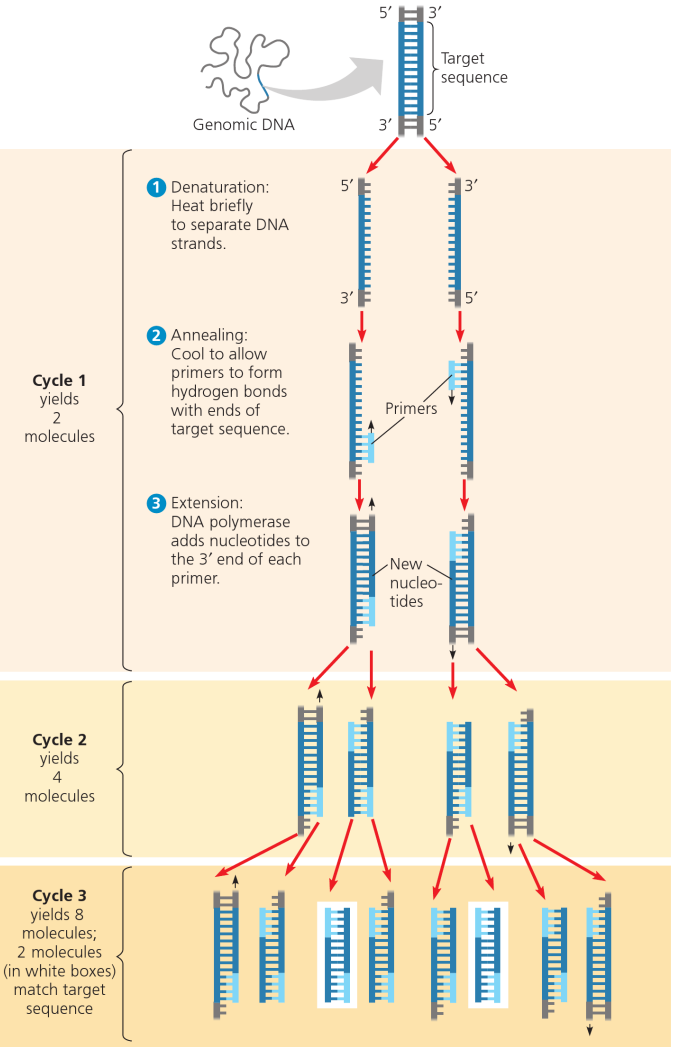
\includegraphics[width=0.7\textwidth]{pcr}
\end{center}
\end{figure}

PCR\ix{Applications} is useful for assays and also provides an alternative to restriction enzymes to forming parts of DNA. \ix{Advantages \& Limitations}PCR is able to isolate fragments independently of restriction sites but there are length constraints on the sequence which PCR can amplify due to the processivity of the polymerase (how quickly the polymerase falls off). Furthermore, the GC content can be an issue for the thermocycling and the polymerase does have an error rate.

PCR can be used to seamlessly join different fragments\ix{Seamless Joining} by \emph{extending primers to create overlaps between PCR reaction products} and then carrying out a PCR reaction on the products (noting that primers are still required because DNA polymerase only works in one direction). Whilst this does allow for seamless joining of arbitrary DNA fragments, only two fragments can be joining at a time and a size limit is imposed by the use of PCR in the final stage.

Several things can go wrong with PCR\ix{What can go wrong?}. Contamination can always be a problem (a laminar air flow hood and filter tips should be used) but assuming fresh, correct buffers \& enzymes and that the thermocycler is correctly programmed, the following are common problems:
\begin{itemize}
\item \underline{No Product}: Check primer design, decrease the annealing temperature (more likely to form base pairs) and try varying \texttt{MgCl\textsubscript{2}} levels.
\item \underline{Multiple Products}: Check primer design! Try using a hot start enzyme (only works at higher temperatures), increasing the annealing temperature and also varying \texttt{MgCl\textsubscript{2}} levels.
\item \underline{Primer Dimers:} The primers self-prime or prime on each each - redesign them!
\item \underline{Incorrect Primer Concentrations:} if too low, the PCR reaction will not work well. 
\end{itemize}

\subsubsection*{Gibson Assembly}
The Gibson Assembly\ix{Gibson Assembly} is a technique for joining DNA molecules which overlap by $\sim 20-40$ base pairs. \ix{Advantages}It is able to combine several DNA fragments with very large lengths ($100+$ kilo-bases) though it is expensive for large lengths. It is cheaper than \emph{de novo} synthesis and fast since it requires few steps and reagents.

\begin{figure}[H]
\begin{center}
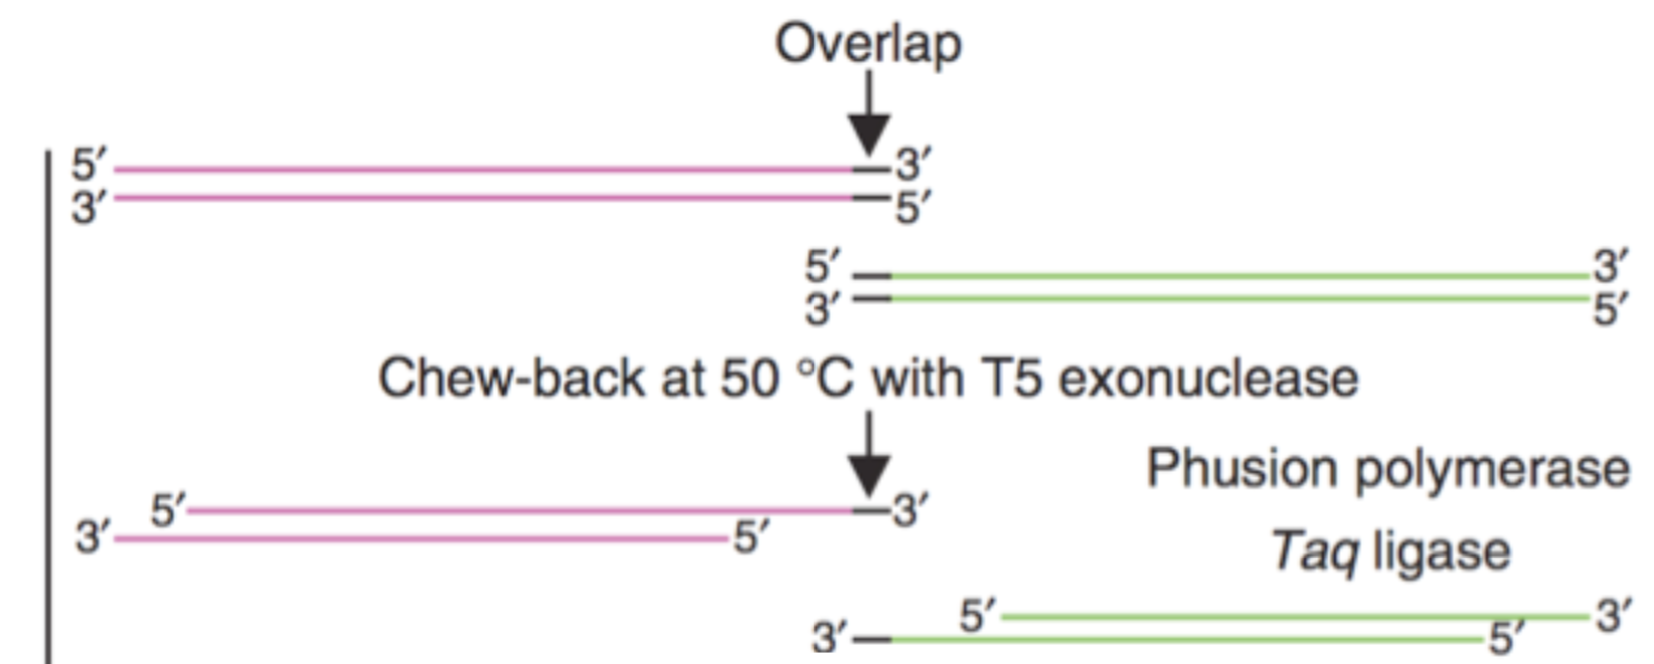
\includegraphics[width=0.7\textwidth]{gibsonAssembly}
\end{center}
\end{figure}

\subsubsection*{\emph{De Novo} Synthesis}
It is also possible to synthesis DNA \emph{de novo}\ix{Advantages} completely independently of restriction sites and ability to PCR. The main limitation of this method is simply cost but this is dropping rapidly. In fact, PCR is not possible without primer synthesis and synthesis of $1$kb is cost effective.

\subsubsection*{CRISPR/Cas9}
CRISPR is a family of DNA sequences in bacteria which contain DNA from viruses which have attacked the bacterium and are used by the bacteria to detect and destroy similar viruses. The CRISPR/Cas9 protein is able to find and cut a DNA target specified by the guide RNA (gRNA) with a specifity of 20 bases and\ix{How to program cut locations?} \textbf{hence by changing the sequence of the gRNA cleavage locations can be programmed} noting that the target must be followed by a \emph{protospacer adjacent motif(PAM)}.

\begin{figure}[H]
\begin{center}
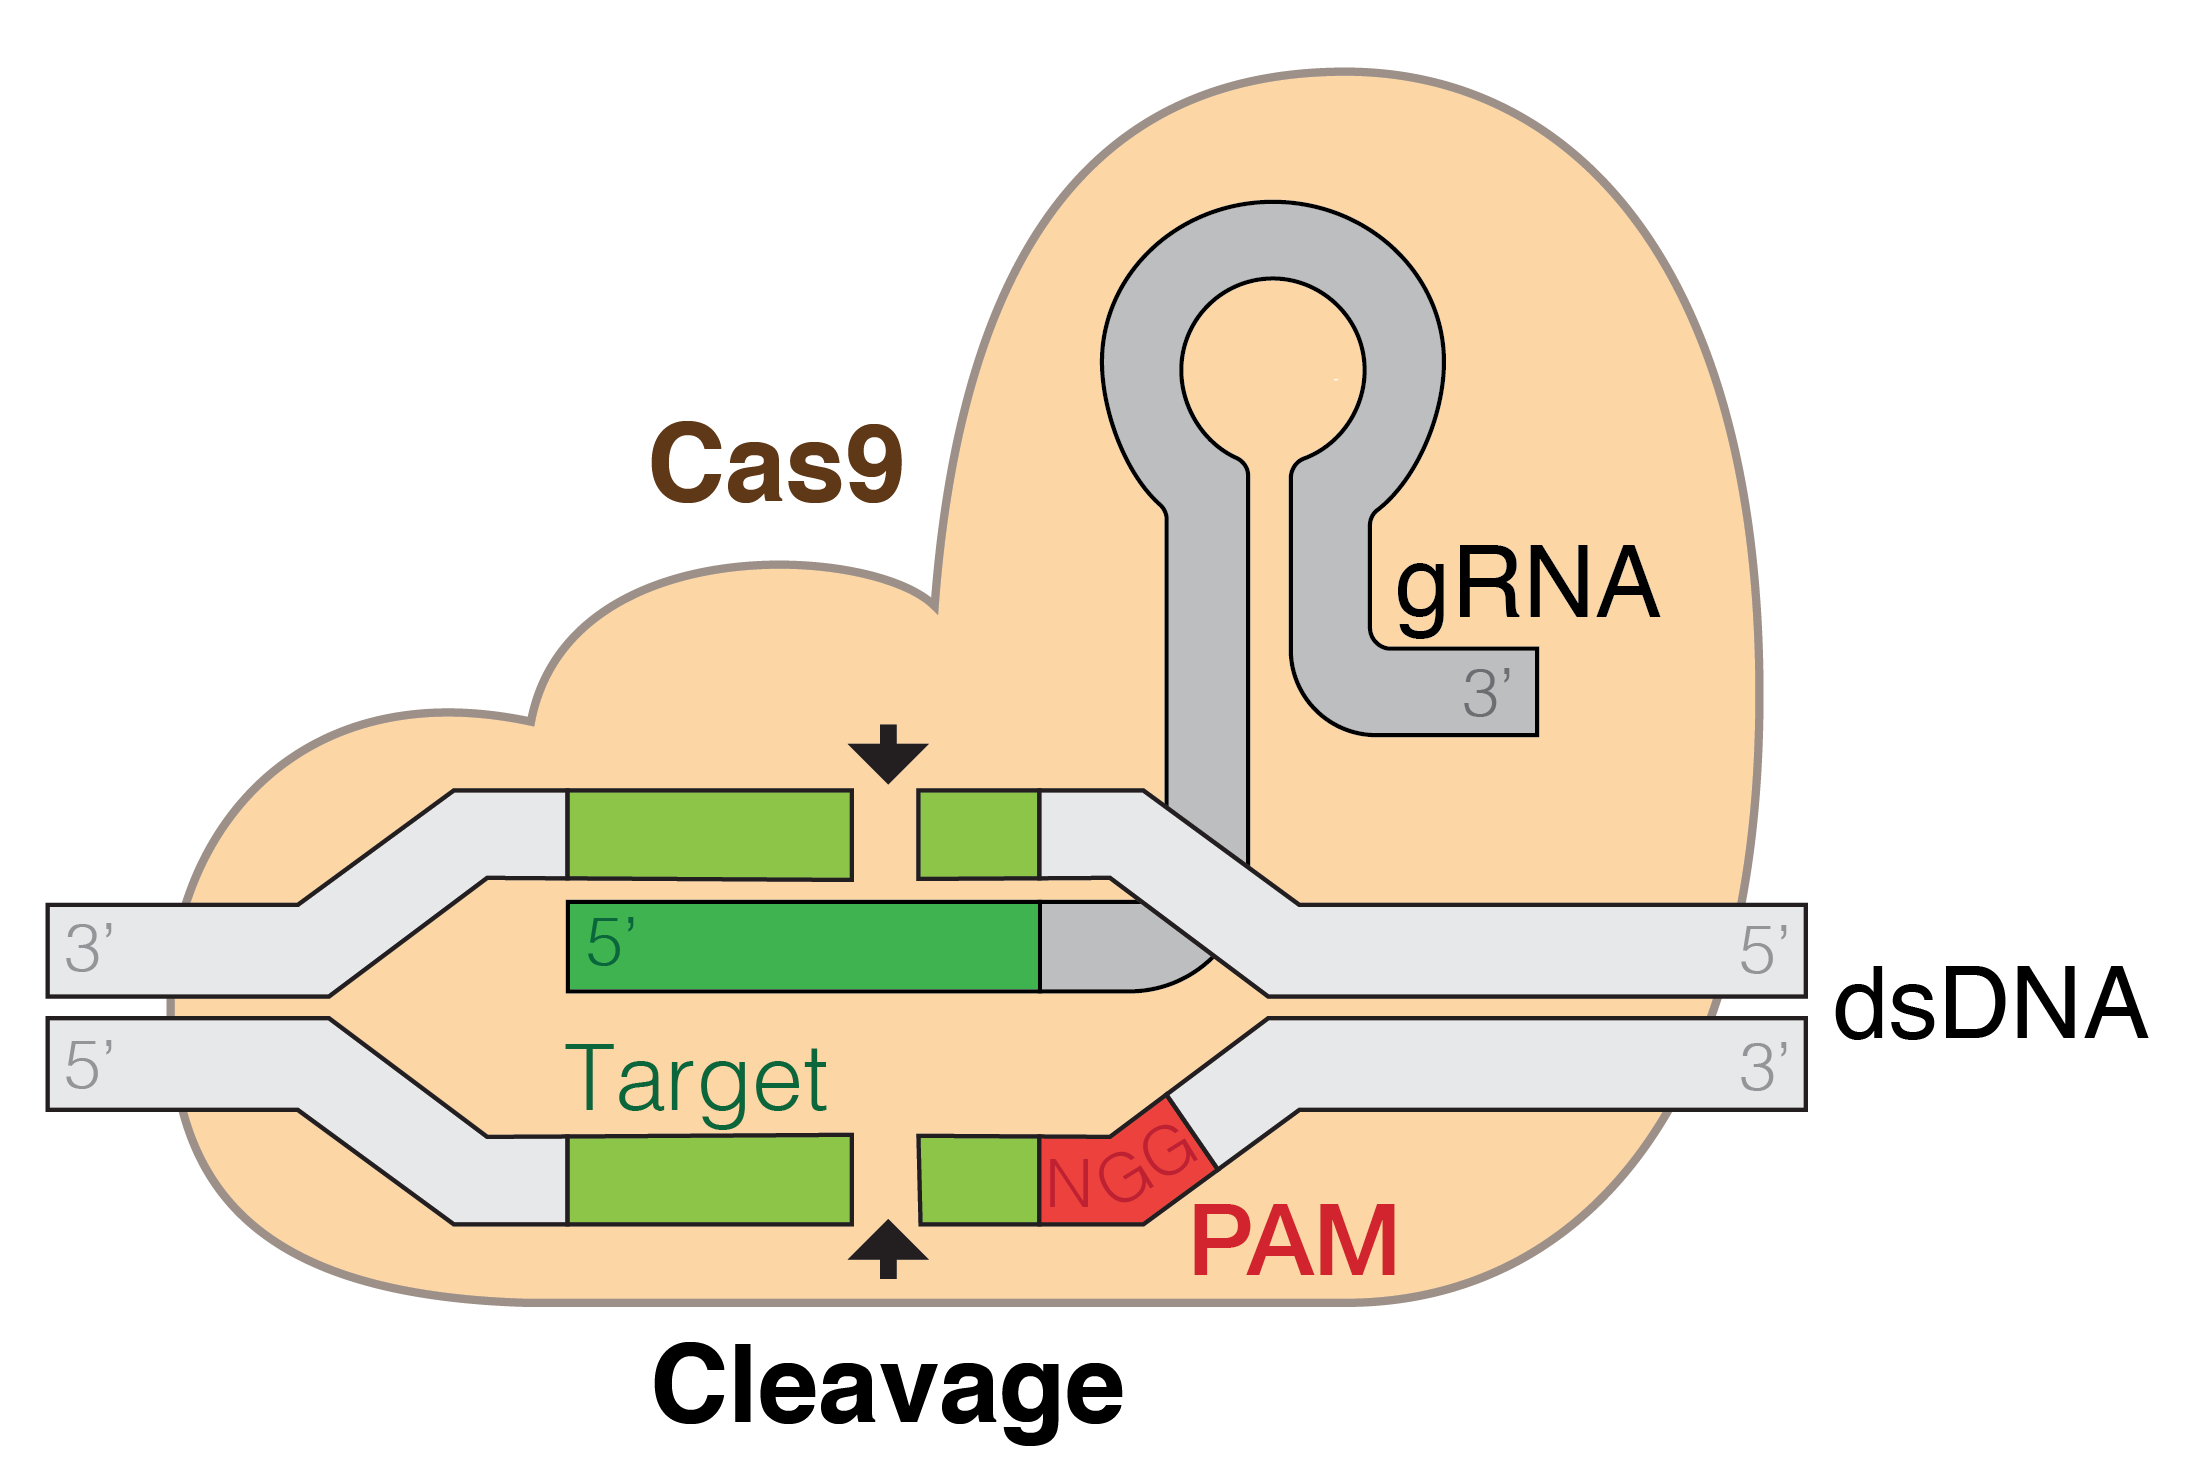
\includegraphics[width=0.5\textwidth]{crispr}
\end{center}
\end{figure}

This allows for homology directed repair.
\begin{figure}[H]
\begin{center}
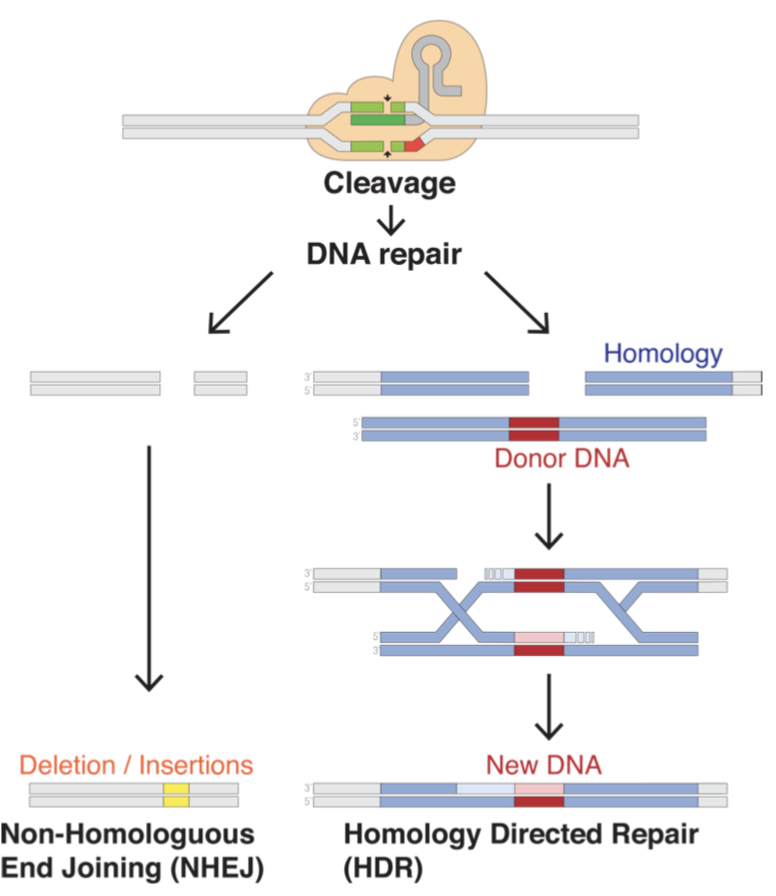
\includegraphics[width=0.5\textwidth]{crisprRepair}
\end{center}
\end{figure}

\subsection{Codon Optimisation}
Since\introduce{Justification?} the amino acid code is redundant, a choice of codons is made when engineering a sequence to express a protein. The codon usage of different organisms is also drastically different e.g. the codon usage in algae and jellyfish is $32\%$ different .

A study\ix{Which codons to use?} in 2009 found that \textbf{favourable codons were predominantly those read by tRNAs that are most highly charged during amino acid starvation}, not the codons which are the most abundant in highly expressed proteins.


\subsection{Case Study: Engineering Insulin}
Insulin is an important human hormone and producing insulin in large quantities is desireable.

Insulin, a hormone produced in the pancreas controls cells through surface receptors. It increases liver, muscle and fat tissue to take up glucose for storage as glycogen and increases fatty acid synthesis. Naturally, insulin creation occurs as follows:\ix{Producing insulin naturally}
\begin{enumerate}
\item Translation into a pro-protein.
\item Folding and oxidiation to form di-sulfide bridges occurs as does signal cleavage.
\item Transportation through the endoplasmic reticulum and the Golgi complex, following by packaging.
\item Central linking fragment is clipped resulting in the two other fragments bound by disulfide bonds, leaving a 51 amino acid monomer.
\end{enumerate}
There are several issues when making insulin:
\begin{itemize}
\item The protein precursor (proprotein) is processed into a mature protein.
\item The signal peptide is cleaved leaving no initiator methionine.
\item The central fragment is cleaved with the polypeptides held with disulfide bonds which need to be formed.
\item Mature insulin is a hexamer with \texttt{Zn} ions; the monomer-hexamer transition can be an issue.
\end{itemize}
The approach taken is to make the two polypeptide chains independently, creating \emph{lacZ-A/B} fusion plasmids which are transformed into \emph{E. coli}. After the beta-galactosidase is removed (from the \emph{lacZ}), each chain is purified, mixed and cross-linked with disulfide bridges.

\subsection{Engineering Antibodies}
It is desirable to produce a specific antibody that can be produced with a high yield. The following is required:\ix{Requirements}
\begin{itemize}
\item High target specificity.
\item Correct self-assembly i.e. folding into an active conformation.
\item The antibody must not itself trigger an immune response.
\item The antibody must be secreted.
\end{itemize}
One method for producing monoclonal antibodies is as outlined in Fig. \ref{fig:makingMabs}. Once the antigen is injected into the mouse, the mouse will produce B cells which secrete the correct anti-bodies. Note that myeloma cells are immortal and the spleen cells contain required B cells meaning that after screening, large batches of the required antibody can be produced.

\ix{The Mouse Method}
\begin{figure}[h!]
\begin{centering}
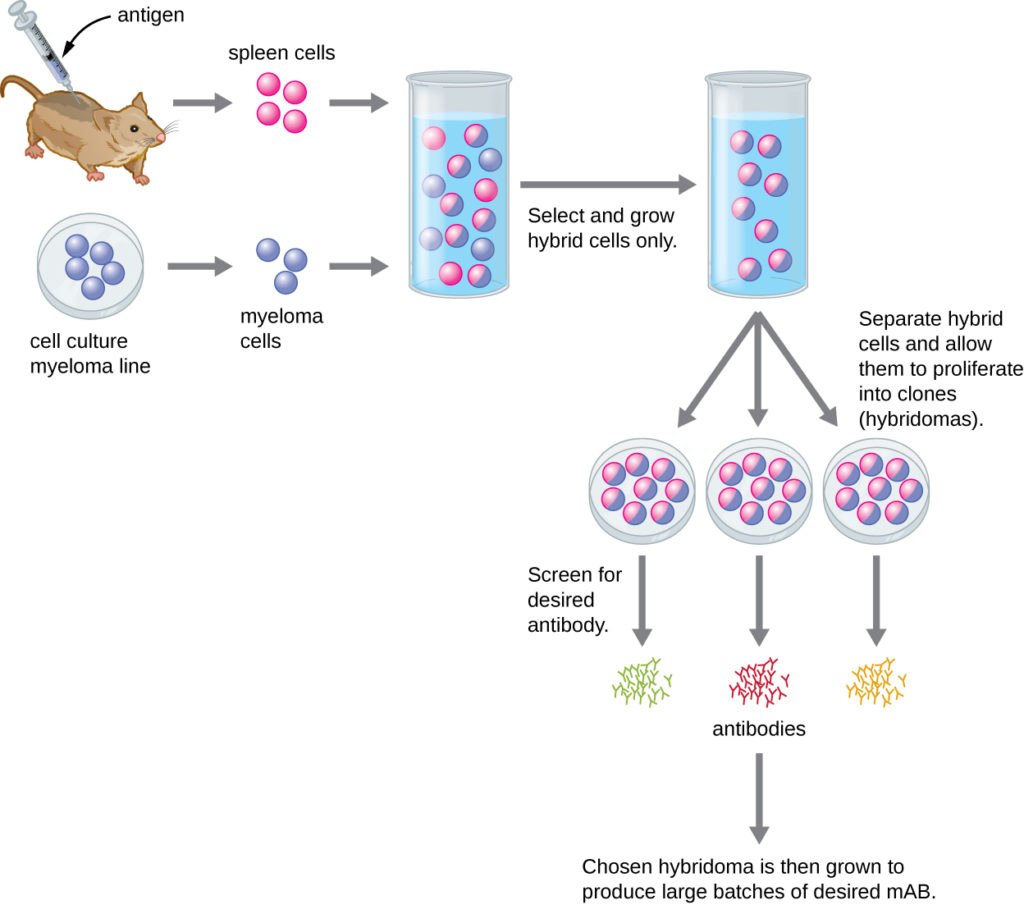
\includegraphics[width=\textwidth]{makeMonoclonal}
\caption{\label{fig:makingMabs} Producing monoclonal antibodies. }
\end{centering}
\end{figure}

The antibodies produced must be humanised \ix{Humanising Antibodies} in order to prevent a immune response. For a humanised anti-body, the hypervariable/CDR regions of the mouse antibody must be combined to the rest of a normal human antibody. There are several ways to humanise antibodies.
\begin{enumerate}
\item CDR grafting uses the above approach, \textbf{replacing the CDR regions} of a human antibody.
\item Alternatively, a mouse carrying human antibody genes can be engineered and the produced antibodies will be human.
\item A more modern technique is to create a \textbf{phage display library} and then select the correct antibody from the library. 
\end{enumerate}

\section{Metabolic Engineering}
\subsection{Preliminaries}
The\ix{Metabolism} metabolism is the network of chemical reactions responsible for the breakdown of molecules for energy (catabolism) and the synthesis of new molecules for cellular function (anabolism). Catabolic bioprocesses are likely to generate energy and produce simpler, smaller building blocks whilst anabolic bioprocesses required energy and produce complex entities.

Precursor metabolites\ix{Precursor Metabolites} are intermediates formed by the catabolism and used by anabolic bioprocesses to form larger molecules. There are 12 precursor metabolites, including: \texttt{glucose-6-phosphate, fructose-6-phosphate, ribose-5-phosphate, pyruvate, ...}

A metabolic pathway\ix{Metabolic Pathway} is a set of reactions interacting under given physiological conditions via (apparently) simple intermediates. An intermediate is simple if there is a single pair of production and consumption reactions.

\subsubsection*{Role of Enzymes}
Metabolic pathways are catalysed by enzymes\ix{Catalysis/Enzymes} which decrease the activation energy of reactions by providing an alternative reaction pathway. The active site of an enzyme is the region where substrate molecules are able to bind and undergo a chemical reaction.

There are two models for the action of enzymes. The lock and key model supposes that the enzyme and substrate are complementary to each other in shape and hence the substrate is also to fit in the enzyme. The induced fit model, there is some distortion of the enzyme as well as the substrate to allow the fit.

\subsubsection*{Linking Between the Catabolism \& Anabolism}
\textbf{Activated carrier molecules}\ix{Activated carrier molecules} serves as energy shuttles, linking the breakdown of food molecules to the energy-requiring synthesis of molecules required by the cell. There are a number of activiated carriers, including the following:

\begin{table}[h!]
\centering
\begin{tabular}{|c|c|}
\hline
Activated Carriers & Group Carried in High-Energy Linkage \\ \hline
\texttt{ATP, GTP}          &  Phosphate                                   \\
\texttt{NADH, NADPH, FADH\textsubscript{2}}                   &   Electrons, Hydrogens \\\hline
\end{tabular}
\caption{Some common activated carrier molecules}
\label{tab:activiatedCarriers}
\end{table}

\ix{Redox Balance}Note that there must be \emph{redox balance} in the cell; every time an electron is lost from a compound (oxidation), an electron must be gained elsewhere (reduction). 

\subsubsection*{Important Pathways}
Glycolysis\ix{Glycolysis} invests two molecules of \texttt{ATP} and a glucose molecule to give a net-gain of two \texttt{NADH \& ATP} molecules as well as two pyruvate molecules. Glucose is converted to fructose which is then cleaved and processed.

The Citric Acid/Krebs cycle is very important\ix{Citric Acid/Krebs cycle}. The bond energy of a pyruvate oxidiation product, acetyl \texttt{CoA}, is harvested to form \texttt{NADH, FADH\textsubscript{2} \& ATP} molecules and the reduced electron carriers can be used to form additional \texttt{ATP}.

In combination, eight of twelve precursors for secreted metabolites are formed from glycolysis and the citric acid cycle and hence these two cycles like at the core of the metabolism.

\subsubsection*{Regulation}
Metabolic pathways can be regulated in different ways.\ix{Types of Regulation}. Hierarchial changes are those caused by changes in enzyme concentration through changes in mRNA processed (i.e. changes in enzyme activities, modifiers) while metabolic changes are those caused by changes in the concentrations of substrates, products or modifiers (changes in substrates, products).
\begin{enumerate}
\item \underline{Mass Action Regulation}\\
The law of mass action proposes that the rate of a chemical reaction is directly proportional to the product of the concentrations of the reactants.

\item \underline{Allosteric Regulation}\\
Allosteric regulation is the regulation of an enzyme by binding an effector molecule at a site other than the enzyme's active site.

\item \underline{Transcriptional Regulation}\\
A \emph{transcription factor} is a protein that controls the rate of transcription by binding to a specific DNA sequence. Transcriptional regulation is where active transcription factors are modified and hence gene expression of enzymes is altered. Can be positive or negative feedback.
\end{enumerate}

\subsubsection*{Enzyme Kinetics}
Enzyme reactions are modeled using the Michaelis-Menten model i.e. a two stage reaction in which the substrate binds first and then the catalytic reaction occurs. \ix{Michaelis-Menten Model}Please see the course notes for \texttt{3G2}.

\subsection{Metabolic Engineering}
\begin{quote}
\centering
The purpose\ix{Purpose} of metabolic engineering is to alter the metabolism of cells to enhance production of native metabolities (metabolism products) or to endow cells with the ability to produce new products.
\end{quote}
Cells are either thought of as a factory which produce products that are deemed to be desirable. Alternatively, the modified cell may be the final product itself. These are a natural example of control loops with feedback and feedforward loops.

\subsubsection*{Building Cell Factories}
When building cell factories\ix{Goal}, the aim is to achieve maximum high quality product secretion (which may require by-product control) at high yield. Several hosts can be used, such as microbes (bacteria and yeast), plants, algae and mammalian cell cultures.

\textbf{Metabolic Flux}\ix{Flux} is defined as the rate of turnover of \textbf{molecules} through a metabolic pathway and hence in essence, we seek to control metabolic fluxes. In order to control fluxes, there are a number of different strategies which can be used:\ix{Strategies}
\begin{itemize}
	\item Alter genes to remove feedback inhibition.
	\item Increase the concentration of key enzymes.
	\item Block metabolic pathways to divert fluxes. 
	\item Introduce genes from other specifies which can create new pathways which can e.g. obtain non-endogenous products. 
\end{itemize}
Note that if exogenous pathways are introduced, it is important to consider the implications of intermediates e.g. whether they are toxic. 
\subsubsection*{Flux Balance Analysis}
Flux balance analysis treats metabolic engineering as a constrained optimisation problem\ix{FBA}. The solution approach is as follows:
\begin{enumerate}
\item Curate metabolic reactions from experimental evidence.
\item Formula the \texttt{\textbf{S}} matrix detailing reaction stoichiometry.
\item Apply the mass-balance constraints (i.e. multiple by a reaction rate vector, \texttt{\textbf{v}} and the steady-state condition).
\item Define an objective function, $Z$, as the dot product between \texttt{\textbf{v}} and a row vector detailing which reactions should be maximised.
\item Optimise $Z$ using linear programming. Note that is it rate to have a single optimal solution point in \texttt{\textbf{v}}.
\end{enumerate}

This approach is not perfect; only one rate-limiting step is present under this regime but in fact, the flux of a pathway can depend on all of the rate constants. Measuring the slowest step (i.e. the step least able to go faster) is not easy.  Each step has some degree of control over the flux.

\subsubsection*{Metabolic Control Analysis}
An alternative to flux balance analysis, metabolic control analysis is a powerful tool. The approach is to use control coefficients which quantity the degree of control each step in a pathway has on the total flux and hence is a system variable; depends on the properties of all enzymes in the system.
\begin{enumerate}
\item Define the \textbf{flux control coefficient}\ix{FCC} as the fractional change in the pathway flux ($J$) caused by a fractional change in the activity of an enzyme ($v$) in that particular pathway. (Note that logs have been taken below).

\begin{equation*}
C_{v_i}^{J} = \frac{d\ \text{ln}\ J}{d\ \text{ln}\ v_i}
\end{equation*}

\item Define the \textbf{concentration control coefficient}\ix{CCC} as the fractional change in metabolite concentration ($S$) cause by a fractional change in the activity of an enzyme producing or consuming that metabolite ($v$).

\begin{equation*}
C_{v_i}^{S} = \frac{d\ \text{ln}\ S}{d\ \text{ln}\ v_i}
\end{equation*}
\end{enumerate}
The above definitions lead to the following summation theorems:
\begin{enumerate}
\item Total control over a metabolic pathway flux should be distributed across all enzymes.\ix{FCC Summation Theorem}
\begin{equation*}
\sum_i C_{v_i}^J = 1
\end{equation*}

\item Control exerted by enzymes whose reactions produce a substrate should be equal to the control exerted by enzymes whose reactions consume that same substrate. \ix{CCC Summation Theorem} (Note different signs)
\begin{equation*}
\sum_i C_{v_i}^S = 0
\end{equation*}

\end{enumerate}
Now, define additional coefficients.
\begin{enumerate}
\item The elasticity coefficient\ix{Elasticity Coefficient} measures the fractional change in the rate of a reaction ($v$) to a fractional change in the concentration of one of its substrates, products or effectors ($S$).
\begin{equation*}
\epsilon_S^v = \frac{\partial\ ln\ v}{\partial\ ln\ S}
\end{equation*}

\item The response coefficient\ix{Response coefficient} measures how the pathway flux ($J$) responds to an effector ($P$)
\begin{align*}
R_P^J = \frac{\partial\ ln\ J}{\partial\ ln\ P} \hspace{1cm} R_P^J = C_{v_i}^J\cdot \epsilon_P^{v_i}
\end{align*}
\end{enumerate}
The connectivity theorems link the kinetic properties of individual reactions to the system properties of a pathway.\ix{Connectivity Theorem} For enzyme, $i$, which responds to a metabolite, $S$,
\begin{align*}
\sum_i C_i^J\cdot \epsilon_S^{i}=0 \hspace{1cm} \sum_i C_i^{S_n}\cdot \epsilon_{S_m}^{i}=0\ \ \ n\neq m\ \text{otherwise -1}
\end{align*}
The\ix{Obtaining FCCs} FCCs of a network cannot be measured directly but are rather inferred by using the connectivity theorem with elasticity measurements.

\subsubsection*{Metabolomics}
The\ix{Metabolome} metabolome refers to the complete set of metabolites present. The transcriptome, proeome and metabolome are all context dependent and vary according to the state of the cell. The metabolome can be profiled by considering what is outside the cell (the exometabolome) but also what is inside the cell (the endometabolome).

The metabolome can be investigated as follows:
\begin{enumerate}
\item Sample collection and preparation.
\item Instrumental analysis e.g. NMR. There are many\ix{Instrumental Difficulties} here; sizes vary over 2 orders of magnitude, abundance varies over many more orders of magnitude. There are also a large number of structural isomers and many metabolites have very different chemical properties (e.g. polarity, volatility).
\item Preprocessing (e.g. noise removal) following by pattern recognition (may be supervised or otherwise).
\item Validation, both statistically and biologically.
\end{enumerate}

\subsubsection*{Overall Method}
In effect, the overall method can be interpreted as follows. A cell culture is analysed (transcriptomics, proteomics and metabolomics) and flux analysis is carried out. Information learn from here is used to alter gene targets and cell strains are then selected and transformation occurs and the cycle repeats. There are some caveats:

\subsection{Biofuels}
There are several generations of Biofuels.
\begin{enumerate}
\item First generation biofuels\ix{1st Gen.} refer to fuels which have been derived from sources such as starch, sugar, animal fats and vegetable oil e.g. biodiesel.

These types of biofuels threaten food supply and biodiversity\ix{Issues} and result in feedstock price volatility. There is also significant issue with the amount of land required.

\item Second generation biofuels\ix{2nd Gen.} are produced from lignocellulosic (plant dry matter), agricultural residues (material left after crops have been harvested) or other forms of waste. The process to produce biofuel with these sources is more complicated but avoids some of the issues with 1st Gen. biofuels. This type of biofuel is very young and there tend to be high capital costs with some domestication issues with certain feedstocks.

\item Third generation biofuels\ix{3rd Gen.} focus on non-arable land e.g. algae or cyanobacteria which require sunlight, \texttt{CO\textsubscript{2}} and water to produce biomass. Similarly there are domestication issues with high capital costs.

\item Fourth generation biofuels\ix{4th Gen.} are similar in technology to the previous generation but \textbf{biomass is not destroyed} e.g. photosynthesis mimicry to produce hydrocarbons.
\end{enumerate}

The choice of feedstock for biofuel creation is important. Different feedstocks will have different proportions of their main sugar substrates and hence will affect the metabolic engineering work required.

\section{Genome Sequencing}
Genome sequencing aids species investigation; it allows finding lesions underlying disease, identifying individual sequence variations and comparing organisms.

\subsection{Genome Structure}
The genome is an organisms complete set of DNA.\ix{What is the Genome?} The structure of the genome is important. The genome of a typical prokaryote is circular with all regions coding for proteins; there is a very high gene density. Eukaryotes have much larger genomes and larger parts of the DNA do not code for RNA or protein.

$95\%$ of the human genome is intergenic sequences. \ix{What's in the Human Genome?} $50\%$ is repetitious regions whilst there are also mobile elements (i.e. selfish DNA which form additional copies of itself within the genome whilst giving no survival advantage). The \texttt{GC} content also varies throughout  and is linked to the gene density. In terms of components, within the genome there are:
\begin{itemize}
\item Protein coding genes.
\item Structural RNA genes e.g. \texttt{rRNA, tRNA}.
\item Regulatory sequences that affect transcription, replication and splicing. Such sequences are controlled by signals which are small $7-20$bp and these signals are often conserved between mechanisms.
\end{itemize}

A genome is made up of\ix{Exons and Introns} exons which code for a protein or peptide sequence and introns which do not code for proteins and interrupt gene sequences.

Across different species, there tends to be conservation\ix{Conservation} of:
\begin{enumerate}
\item Gene order.
\item Regulatory Motifs.
\item Protein sequence. Hence most changes tend to be \textbf{conservative} e.g. changing the codon which is used but not the amino acid sequence.
\end{enumerate}
Often in smaller genomes of different species, significant portions of the repeating regions have been lost. Note that when comparing different genomes, gene number is a poor method of assessing complexity.

\subsection{Sequencing Techniques}
\subsubsection*{Sanger DNA Sequencing}
Sanger DNA\ix{Sanger DNA Sequencing ingredients} sequencing is able to sequence up to about 900 base pairs. The technique requires the following ingredients:
\begin{enumerate}
\item A DNA Polymerase enzyme.
\item DNA Nucleotides, \texttt{dATP, dTTP, dCTP, dGTP}.
\item A DNA Primer.
\item Population of the DNA template to be sequenced; a population of a molecule only gives one read. 
\item \textbf{Dideoxy}\ix{\texttt{ddNTP}} versions of each nucleotide e.g. \texttt{ddATP} \textbf{each labeled with a different dye}.

\begin{figure}[H]
\begin{centering}
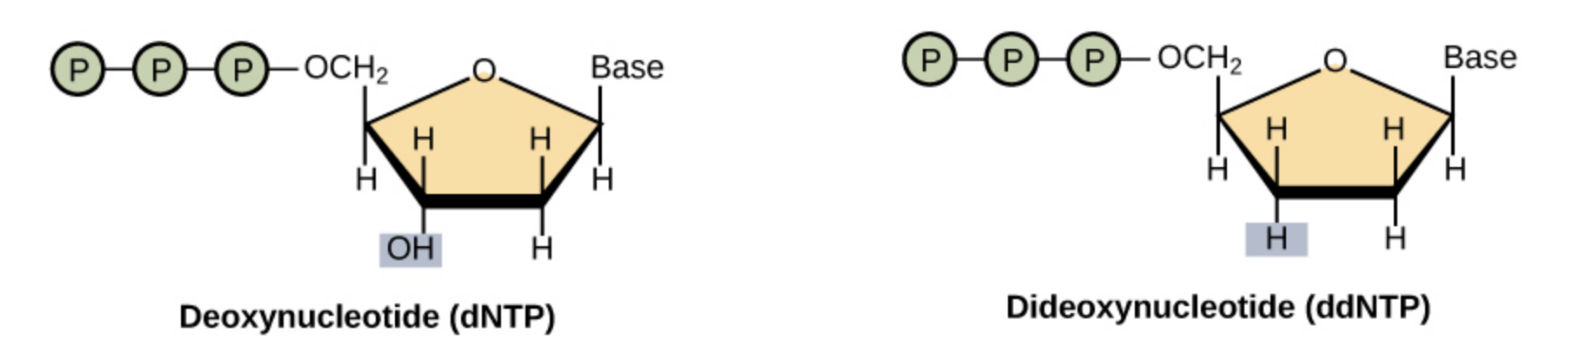
\includegraphics[width=0.6\textwidth]{ddNtp}
\caption{\label{fig:ddNtp} Dideoxy nucleotide versions.}
\end{centering}
\end{figure}
Once a dideoxy nucleotide has been added to a chain, there is no hydroxyl group available and hence no further nucleotides can be added. The chain ends with a \textbf{dyed nucleotide}.
\end{enumerate}
Hence,\ix{Method} a the DNA sampled is heated to anneal the DNA and cooled to allow the primer to bind. The temperature is raised to allow DNA polymerase to synthesise new DNA and it is virtually guaranteed that a dideoxy nucleotide will be at every position of the DNA. Gel electrophoresis is used to separate out the molecules and hence the sample can be sequenced.

Whilst this method gives high-quality sequencing, it is expensive, time consuming\ix{Evaluating Sanger} and inefficient for sequencing larger projects e.g. the whole genome.

\subsubsection*{Next Generation Sequencing}
Next generation sequencing, such as Illumina, is able to read far faster than Sanger sequencing. See \url{https://www.youtube.com/watch?v=fCd6B5HRaZ8} for an excellent video. Fig. \ref{fig:illumina} outlines the general method for this technology but the important points are important:
\begin{itemize}
\item Adapters\ix{Adapters: Why?} to each DNA fragment are added which not only allow reuse of the same primer but also allow sample identification.
\item After bridge amplification, only the forward strands are kept. After the read, bridge amplification occurs again and the same strand is then read again backwards.
\item Many sequences are sequenced at once.
\item There are about 1000 copies of DNA in each cluster; this aids digital imaging.
\item Computer controlled imaging is used to sequence millions of clusters in parallel.
\item \textbf{Crucially, the bases are extended by one base each step} after the primers have annealed with different colours corresponding to different bases.\ix{Extending one bases at a time} This is achieved by using dyed \texttt{NTPs} which cannot be extended. After imaging, the terminator and dye are cleaved from the \texttt{NTP} and then extended by an additional base pair.
\end{itemize}

\begin{figure}[H]
\begin{centering}
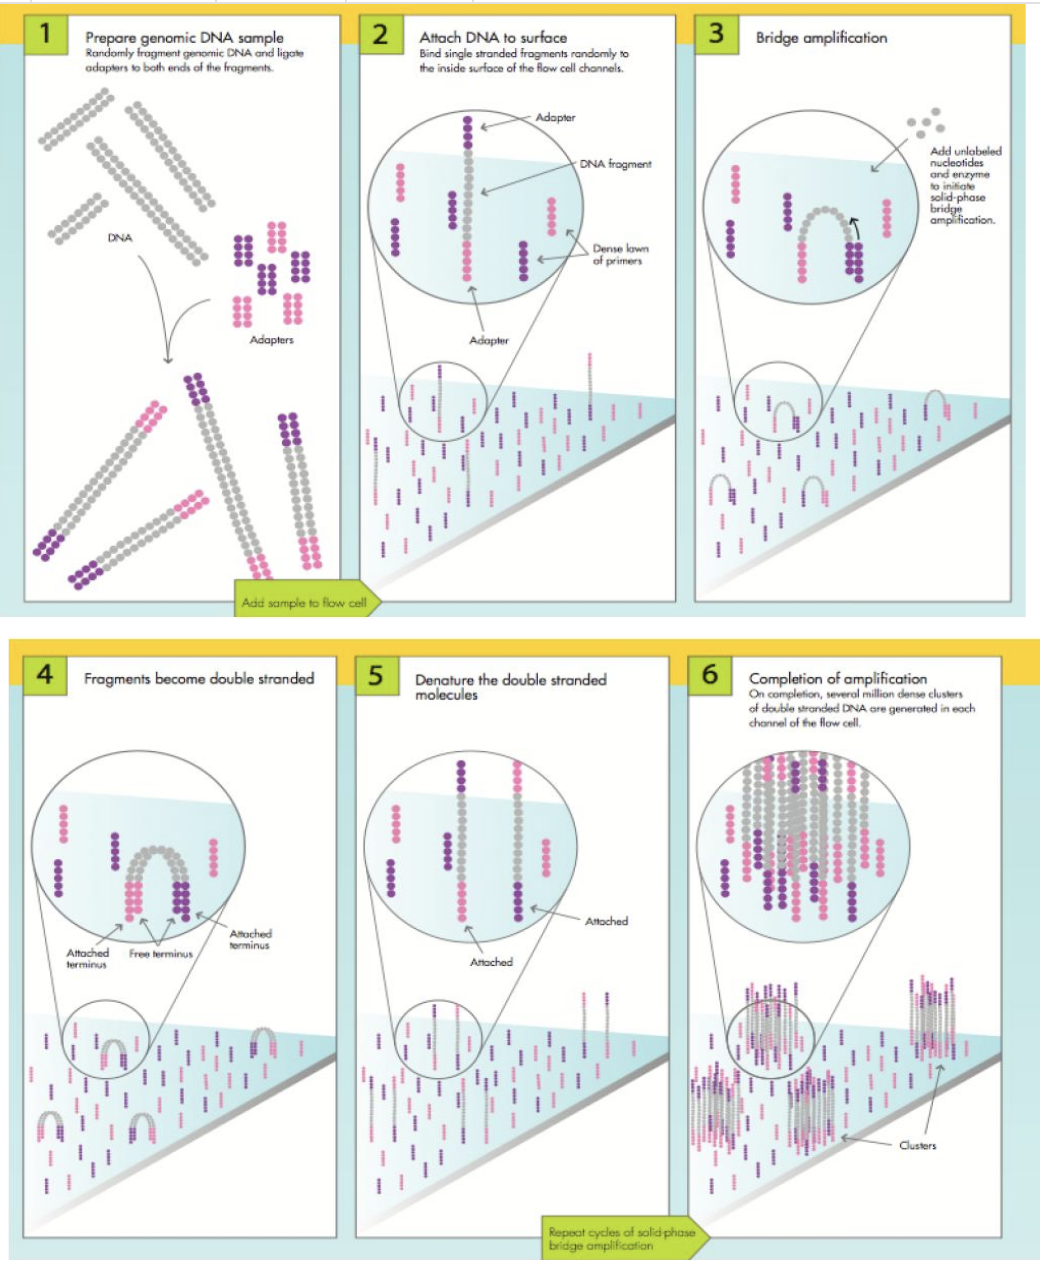
\includegraphics[width=0.8\textwidth]{illumina}
\caption{\label{fig:illumina} Illumina: A Next Generation sequencing technology.}
\end{centering}
\end{figure}

Compared to Sanger sequencing, Illumina sequencing does have a shorter read length but there are $3000\cdot 10^6$ reads per run and $300\cdot 10^9$ bases per single end run. Unlike the Sanger method, each sequence corresponds to a read. It is expensive and time consuming; the `sequencing by synthesis step' can take up to 8 days and the software analysis up to 2 days.

\subsection{Whole Genome Sequencing}
A genome of say $10^9$ bases is hard to sequence when only a limited number of bases can be read at a time. One approach is to:
\begin{enumerate}
\item Fragment the genome.
\item Sequence the fragments.
\item Assemble the genome by searching for overlapping fragments.
\end{enumerate}

\subsubsection*{Whole Genome Shotgun Sequencing}
Initially controversial, this is now the standard approach.\ix{Shotgun Sequencing} DNA is broken up randomly into numerous small sequences which can then be sequenced e.g. using the Sanger method. \textbf{Several rounds of fragmentation and sequencing} are performed leading to multiple overlapping reads for the target DNA and the overlapping reads can then be assembled into a continuous sequence (through software).

There are issues:\ix{Problems?} there is a cloning bias since different DNA fragments have different affinities for cloning and assembly has potential for huge mistakes with difficult repeating systems and was computationally hard.

\subsection{Libraries}
A\ix{Library} library is a collection of \textbf{cloned} DNA fragments; each clone is fused with a vector (often a plasmid) and can be transformed into host cells. Vector sequences can be used for selection of cells which contain cloned DNA. A `good' library has the following properties:
\begin{itemize}
\item Even source material representation.
\item Few empty vectors.
\item DNA not rearranged.
\item No vectors with multiple inserts.
\end{itemize}

Libraries are made\ix{Production} by isolating the desired fragments and then ligating them into a vector. Two common libraries are cDNA libraries (gene libraries produced using a reverse transcriptase enzyme which copies mRNA to DNA) and genomic DNA. Source fragments can be synthesised, creating using different restriction enzymes or randomly sheared.

There is a maximum insert size since a larger insert tends to decrease stability and give a poor transformation efficiency. Cosmid inserts can give $\sim 30$kb inserts whilst more modern bacterial artificial chromosome inserts give around $100-150$kb inserts.

\subsection{Finding Genes}
There are multiple approaches to finding genes once a genome has been sequenced.\ix{Approaches}
\begin{itemize}
\item Human and vertebrate \texttt{cDNA} (complementary DNA formed from single stranded \texttt{mRNA} in a reaction catalysed by reverse transcriptase) can be aligned to the genome.
\item The genome can be compared to known protein, finding similarities.
\item \emph{Ab initio} i.e.\ using statistical gene finders.
\end{itemize}

\subsection*{Sequence Alignment}
Sequence alignment is very important across molecular bioengineering.\ix{Why important?} It it often used to
\begin{itemize}
\item match mRNA to genome sequence and match protein sequences to a genome.
\item find overlapping sequences required for genome sequence assembly.
\item find where PCR primers may be mis-priming.
\item identify families of related protein sequences.
\end{itemize}

To develop methods of aligning sequences, the presence of gaps and amino-acid substitutions must be considered.

Amino-acid substitutions are scored using the log-likelihood with a large set of high quality ungapped protein sequence alignments.
\begin{align*}
\text{score}(a, b) = \text{log}(\frac{p_{ab}}{p_a p_b})
\end{align*}
The log likelihood score is positive if aligned more often than expected and vice versa. The score is often rounded to the nearest integer for computational efficiency.

Gaps tend to occur in runs. There are different penalities which can be used to score gaps. For a gap length of $g$, the following scoring methods are often used:
\begin{align*}
\text{Linear: penalty} &= -d \cdot g \\
\text{Affine: penalty} &= -d - e(g-1) \hspace{1cm} e < d
\end{align*}
In the linear case, $d$ acts a per-residue gap penalty. In the affine case, there is a larger price to pay for `opening' a gap and hence an extension penalty is used which is lower.

\subsubsection*{Dynamic Programming}
It\ix{Dotter} is possible to compare every residue in one sequence to every residue in another i.e. check every possible alignment. In time and memory, for sequences of length $M$ and $N$, the complexity is $O(M\times N)$. Diagonal lines indicate matching sequences but this does not allow for gaps. An alignment with gaps will have a downwards and rightward trend but note that there \textbf{may be a gap in either of the sequences}.

To account for gaps, dynamic programming is used. \ix{Algorithm Steps}
\begin{enumerate}
\item Fill out a matrix of scores with each cell maximising its score by examining the three already evaluated neighbours. It will inherit the neighbours score and either pay a penalty for a gap or increase in score due to a good alignment.

\begin{figure}[H]
\begin{center}
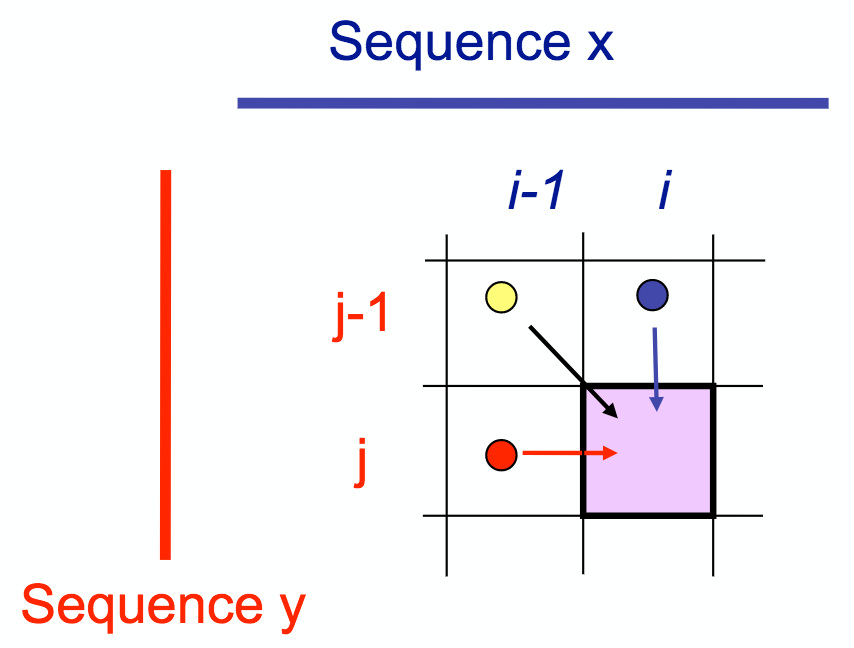
\includegraphics[width=0.4\textwidth]{dynamic1}
\caption{$F(i,j)$ is the score of the best alignment of subsequences $(x_1, x_2, ... x_i)$ and $(y_1, y_2, ... y_j)$. The algorithm is recursive and depends on previously evaluated values.}
\end{center}
\end{figure}


\begin{align*}
F(i, j) = \max \begin{cases}
F(i-1, j-1) + \text{score}(x_i, y_j) \\
F(i, j-1) - d\\
F(i-1, j) - d
\end{cases}
\end{align*}
For each cell, a traceback pointer records from which parent the best score was inherited.

\item To generate the alignment, each traceback point is followed backwards from the final cell evaluated.
\end{enumerate}
This algorithm has the same complexity as the dotter. There are many variants such as the best overlap, best local alignment and there are linear memory variants of the algorithm.  An alignment can be considered to be a path through a finite state machine.

\ix{Using this in practice}This technique is used to find genes by aligning \texttt{cDNA} and can also be used to search for proteins. However, there are huge gaps and the method must be tolerant. Since this would be costly to solve via dynamic programming, dynamic programming is used to piece exons \textbf{once they have been roughly located using heuristic methods}.

\subsection*{\emph{Ab Initio} Gene Finding: GenScan}
GenScan simultaneously finds forward and reverse genes. It is a probabilistic model which includes models for exons with $O(\text{States} \cdot M)$ (which is very fast). \ix{Complexity}However, nested genes are missing and there is no alternate splicing.

Similarly to dynamic programming, this model can be represented as a finite state machine but is far more complex. The FSM is symmetric since the model is able to read genes from the forward and reverse strand simultaneously. The model effective chooses genes which align best with model evidence and many heuristics are used.

\subsection{Investigating a Gene}
There are many methods\ix{Investigating Genes} for investigating genes. Directed approaches include removing the gene, over-amplifying it or directing mutation of the gene. Alternatively, random mutagenesis can be used (i.e.\ change the genome and screen for phenotypes) or error-prone PCR used to randomly alter specific regions of DNA\@. In fact,\ix{RNAi} RNA can be used to repress genes through RNA interference; \texttt{dsRNA} is expressed as smaller interfering RNA binds to \texttt{mRNA}. Alternatively, CRISPR/Cas9 can also be used for gene knockout.


\end{document}
